\chapter{Complex Numbers and Polynomials}
By definition a complex number has two parts: a real part and an imaginary part. You already know about real numbers and know about
them. However, imaginary numbers is something different.
\section{Imaginary Numbers}
Imaginary numbers are called so because there cannot be physical representation of these quantities. Like we use real numbers for
counting physical objects we cannot do that with imaginary numbers. In real world, they do not exist. Square root of negative
numbers are called imaginary numbers. For example, $\sqrt{-1}, \sqrt{-2}. \sqrt{-3}, \ldots$ and so on.

We denote $\sqrt{-1}$ with the Greek symbol $\iota$, which stands for \textit{iota}. We also use English letters \textit{i} or
\textit{j} to represent this imaginary number. Clearly, $i^2 = -1, i^3 = -i, i^4 = 1$. If you examine carefully, you will find that
following holds true:

$$i^{4m} = 1, i^{4m + 1} = i, i^{4m + 2} = -1 \text{~and~} i^{4m +3} = -1, \forall m\in P$$

\dangersign \textbf{Gotcha:}

Consider the following:

$$1 = \sqrt{1} = \sqrt{-1*-1} = \sqrt{-1}*\sqrt{-1} = i*i = -1$$

However, the above result is wrong. The reason being is that for any two real numbers $a$ and $b, \sqrt{a}*\sqrt{b} = \sqrt{ab}$
holds good if and only if two numbers are either zero or positive. Also, $\sqrt{1}\neq \sqrt{-1*-1}$ because power of $-$ is
$\frac{1}{2}$ which results in $-1$.

\section{Definitions Related to Complex Numbers}
A complex number is written as $a + ib$ or $x + iy$ or $a + jb$ or $x + jb$. Here, $a, b, x, y$ are all real numbers. The complex
numbers itself is denoted by $z$. Therefore, we have $z = x + iy$. Here, $x$ is called the real part and is also denoted by $\Re(z)$
and $y$ is called the imaginary part and is also denoted by $\Im(z)$.

A complex number is purely real if its imaginary part or $y$ or $\Im(z)$ is zero. Similarly, a complex number is purely imaginary if
its real part or $x$ or $\Re(z)$ is zero. Clearly, as you can imagine that there can exist only one number which has both the parts
as zero and certainly that is $0$. That is, $0=0+i0$.

The set of all complex number is typically denoted by $C$. Two complex numbers $z_1$ and $z_2$ are said to be true if there real
parts are equal and imaginary parts are equal. That is if $z_1=x_1+iy_1$ and $z_2=x_2+iy_2$ then $x_1$ must be equal to $x_2$ and
similarly for imaginary part for two complex numbers to be equal.

\section{Simple Arithmetic Operations}
\subsection{Addition}
$(a + ib) + (c + id) = (a + c) + i(b + d)$
\subsection{Subtraction}
$(a + ib) - (c + id) = (a - c) + i(b - d)$
\subsection{Multiplication}
$(a + ib) * (c + id) = ac + ibc + iad + bdi^2 = (ac - bd) +i(bc + ad)$
\subsection{Division}
The complex number in denominator must not have both parts as zero. At least one part must be non-zero.

$$\frac{a + ib}{c + id} = \frac{(a + ib)(c - id)}{(c + id)(c -id)} = \frac{(ac + bd) + i(bc -ad)}{c^2+d^2}$$

\section{Conjugate of a Complex Number}
Let $z = x + iy$ be a complex number then its complex conjugate is a number with imaginary part made negative. It is written as
$\overline{z} = x - iy. \overline{z}$ is the typical representation for conjugate of a complex number $z$.

\subsection{Properties of Conjugates}
\begin{enumerate}
\item $z_1 = z_2 \Leftrightarrow \overline{z_1} = \overline{z_2}$

  Clearly as we know for two complex numbers to be equal, both parts must be equal. So this is very easy to understand that if $x_1
  = x_2$ and $y_1 = y_2$ then this bidirectional condition is always satisfied.
\item $\overline{\left(\overline{z}\right)} = z$

  $z = x + iy$, hence, $\overline{z} = x - iy$. Hence, $\overline{\left(\overline{z}\right)} = x - (-iy) = x + iy = z$
\item $z + \overline{z} = 2\Re(z)$

  $z + \overline{z} = x + iy + x - iy = 2x = 2\Re(z)$.
\item $z - \overline{z} = 2i\Im(z)$

  $z - \overline{z} = x + iy - (x - iy) = 2iy = 2i\Im(z)$
\item $z = \overline{z} \Leftrightarrow z$ is purely real.

  Clearly, $x + iy = x - iy \Rightarrow 2iy = 0 \Rightarrow y = 0$. Therefore, $z$ is purely real. Conversely, if $z$ is purely
  real then $z = x$, and thus $z = \overline{z}$.
\item $z + \overline{z} = 0 \Leftrightarrow z$ is purely imaginary.

  Clearly, $x + iy + x - iy = 0 \Rightarrow 2x = 0$. Therefore, $z$ is purely imaginary. Conversely, if $z$ is purely imaginary
  then $z = iy$, and thus $z + \overline{z} = 0$.
\item $z\overline{z} = [\Re(z)]^2 + [\Im(z)]^2$

  Clearly, $z\overline{z} = (x + iy)(x - iy) = x^2 + y^2 = [\Re(z)]^2 + [\Im(z)]^2$
\item $\overline{z_1 + z_2} = \overline{z_1} + \overline{z_2}$

  $\overline{z_1 + z_2} = \overline{(x_1 + iy_1) + (x_2 + iy_2)} = \overline{(x_1 + x_2) + i(y_1 + y_2)} = (x_1 + x_2) - i(y_1 +
  y_2) = (x_1 - iy_1) + (x_2 - iy_2) = \overline{z_1} + \overline{z_2}$
\item $\overline{z_1 - z_2} = \overline{z_1} - \overline{z_2}$

  This can be proven like previous item.
\item $\overline{z_1z_2} = \overline{z_1}\overline{z_2}$

  This can be proven like previous item.
\item $\overline{\left(\frac{z_1}{z_2}\right)} = \frac{\overline{z_1}}{\overline{z_2}}$ if $z_2\neq 0$

  It can be proven by multiplying and dividing by conjugate of denominator and then applying division formula given above.
\item If $P(z) = a_0 + a_1z + a_2z^2 + \ldots + a_nz^n$, where $a_0, a_1, \ldots, a_n$ and $z$ are complex numbers, then

  $$\overline{P(z)} = \overline{a_0} + \overline{a_1}(\overline{z}) + \overline{a_2}(\overline{z})^2 +
  \overline{a_n}(\overline{z})^n = \overline{P}(\overline{z})$$

  where

  $$\overline{P}(z) = \overline{a_0} + \overline{a_1}z + \overline{a_2}z^2 + \ldots + \overline{a_n}z^n$$
\item If $R(z) = \frac{P(z)}{Q(z)}$, where $P(z)$ and $Q(z)$ are polynomials in $z$, and$Q(z) \neq 0$, then

  $$\overline{R(z)} = \frac{\overline{P}(\overline{z})}{\overline{Q}(\overline{z})}$$
\item If $$z = \begin{vmatrix}a_1 & a_2 & a_3\\ b_1 & b_2 & b_3 \\ c_1 & c_2 & c_3\end{vmatrix}, \text{~then~}\overline{z}
  = \begin{vmatrix}\overline{a_1} & \overline{a_2} & \overline{a_3}\\ \overline{b_1} & \overline{b_2} & \overline{b_3}
    \\ \overline{c_1} & \overline{c_2} & \overline{c_3}\end{vmatrix},$$
  where $a_i, b_i, c_i(i = 1,2,3)$ are complex numbers.
\end{enumerate}

\section{Modulus of a Complex Number}
Modulus of a complex number $z$ is denoted by $|z|$ and is equal to the real number $\sqrt{x^2 + y^2}$. Note that $|z| \geq
0~\forall z \in C$.
\subsection{Properties of Modulus}
\begin{enumerate}
\item $|z| = 0 \Leftrightarrow z = 0$

  Clearly, this means $x^2 + y^2 = 0 \Rightarrow x = 0$ and $y = 0 \Rightarrow z = 0$.
\item $|z| = |\overline{z}| = |-z| = |-\overline{z}|$

  Clearly, all result in $\sqrt{x^2 + y^2}$.
\item $-|z| \leq \Re(z) \leq |z|$.

  Clearly, $-\sqrt{x^2 + y^2}\leq x\leq \sqrt{x^2 + y^2}$.
\item $-|z| \leq \Im(z) \leq |z|$.

  Clearly, $-\sqrt{x^2 + y^2}\leq y\leq \sqrt{x^2 + y^2}$.
\item $z\overline{z} = |z|^2$

  Clearly, $(x + iy)(x - iy) = x^2 + y^2 = |z|^2.$
\end{enumerate}

\noindent Following relations are very easy and can be proved by the student. If $z_1$ and $z_2$ are two complex numbers then,

\begin{enumerate}[resume]
\item $|z_1z_2| = |z_1||z_2|$

  $|z_1z_2| = |x_1x_2 - y_1y_2 + i(x_1y_2 + x_2y_1)| = \sqrt{(x_1x_2 - y_1y_2)^2 + (x_1y_2 + x_2y_1)^2} = \sqrt{(x_1 + y_1)^2(x_2 +
  y_2)^2} = |z_1||z_2|$
\item $\left|\frac{z_1}{z_2}\right| = \frac{|z_1|}{|z_2|}$ if $z_2\neq = 0$
\item $|z_1 + z_2|^2 = |z_1|^2 + |z_2|^2 + \overline{z_1}z_2 + z_2\overline{z_2} = |z_1|^2 + |z_2|^2 + 2\Re(z_1\overline{z_2})$.
\item $|z_1 - z_2|^2 = |z_1|^2 + |z_2|^2 - \overline{z_1}z_2 - z_1\overline{z_2} = |z_1|^2 + |z_2|^2 + 2\Re(z_1\overline{z_2})$.
\item $|z_1 + z_2|^2 + |z_1 - z_2|^2 = 2\left(|z_1|^2 + |z_2|^2\right)$.
\item If $a$ and $b$ are real numbers, and $z_1$ and $z_2$ are complex numbers, then

  $|az_1 + bz_2|^2 + |bz_1 - az_2|^2 = (a^2 + b^2)\left(|z_1|^2 + |z_2|^2\right)$.
\item If $z_1, z_2\neq = 0$, then $|z_1 + z_2|^2 = |z_1|^2 + |z_2|^2 \Leftrightarrow \frac{z_1}{z_2}$ is purely imaginary.
\item If $z_1$ and $z_2$ are complex numbers then $|z_1 + z_2| \leq |z_1| + |z_2|$. This inequality can be generalized to more
  terms as well.
\item $|z_1 - z_2| \leq |z_1| + |z_2|, ||z_1| - |z_2||\leq |z_1| + |z_2|$ and $|z_1 - z_2|\geq ||z_1| - |z_2||$. These are trivial
  to prove.
\end{enumerate}

\section{Geometrical Representation}
A complex number $z$ which we have considered to be equal to $x+iy$ in our previous representations can be represented by a point
$P$ whose Cartesian coordinates are $(x,y)$ referred to rectangular axes $Ox$ and $Oy$ where $O$ is origin i.e. $(0, 0)$ and are
called \textit{real} and \textit{imaginary} axes respectively. The $xy$ two-dimensional plane is also called \textit{Argand plane,
complex plane} or \textit{Gaussian plane}. The point $P$ is also called the image of the complex number and $z$ is also called
the \textit{affix} or \textit{complex coordinate} of point $P$.

Now as you can easily figure out that all real numbers will lie on real axis and all imaginary numbers will lie on imaginary axis
as their counterparts will be zero.

The modulus is given by the length of segment $OP$ which is equal to $OP=\sqrt{x^2+y^2}=|z|$. This, $|z|$ si the length of the
$OP$. Given below is the graphical representation of the complex number.

\begin{figure}[H]
  \begin{center}
    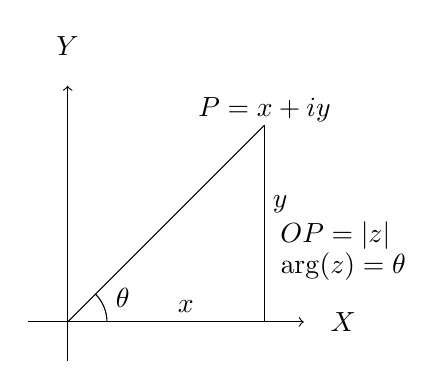
\begin{tikzpicture}
      \draw[->] (-.5,0) -- (3,0);
      \draw[->] (0,-.5) -- (0,3);
      \draw (0, 3.5) node {$Y$};
      \draw (3.5, 0) node {$X$};
      \draw (2.5,0) -- (2.5,2.5);
      \draw (0,0) -- (2.5, 2.5);
      \draw (.5,0) arc(0:45:.5);
      \draw (.7,.3) node{$\theta$};
      \draw (1.5, 0.2) node {$x$};
      \draw (2.7, 1.5) node {$y$};
      \draw (3.4, 1.1) node {$OP=|z|$};
      \draw (3.5, 0.7) node {$\arg(z)=\theta$};
      \draw (2.5, 2.7) node{$P=x+iy$};
    \end{tikzpicture}
    \caption{Complex number in argand plane or complex plane}
  \end{center}
\end{figure}

In the diagram, $\theta$ is known as the \textit{argument} of $z$. This is nothing but angle made with positive direction
(i.e. counter-clockwise) of real axis. Now, this argument is not unique. If $\theta$ is an argument of a complex number $z$ then,
$2n\pi + theta$, where $n\in I$, where I is the set of integers. The value of argument for which $-\pi<\theta\leq \pi$ is called
the \textit{principal value} of \textit{argument} or \textit{principal argument}.

\subsection{Different Arguments of a Complex Number}
In the diagram, the argument is given as $\\arg(z) = \tan^{-1}\left(\frac{y}{x}\right)$, this value is for when $z$ in first
quadrant. When $z$ will lie in second, third and fourth quadrants the arguments will be
$$\\arg(z) = \pi - \tan^{-1}\left(\frac{y}{|z|}\right), \arg(z)= -\pi + \tan^{-1}\left(\frac{|y|}{|z|}\right)\text{~and~} \arg(z) =
-\tan^P{-1}\left(\frac{|y|}{x}\right)$$
respecticely.

\subsection{Polar Form of a Complex Number}
If $z$ is a non-zero complex number, then we can write $z = r(\cos\theta + i\sin\theta)$, where $r = |z|$ and $\theta = \arg(z)$.

In this case, $z$ is also given by $z = r[\cos(2n\pi  \theta) + i\sin(2n\pi + \theta)]$, where $n\in I$.

\subsubsection{Euler's Formula}
The complex number $\cos\theta + i\sin\theta$ is denoted by $e^{i\theta}$ or $c$ is $\theta$, where $c$ is the complex number.

\subsection{Important Results Involving Arguments}
If $z, z_1$ and $z_2$ are complex numbers, then

\begin{enumerate}
\item $\arg(\overline{(z)}) = -\arg(z)$. This can be easily proven as if $z = x + iy$, then $\overline{z} = x - iy$ i.e. sign of
  argument will get a -ve sign as $y$ gets one.
\item $\arg(z_1z_2) = \arg(z_1)  + \arg(z_2) + 2n\pi$, where
  $$n = \begin{cases}
   0 \text{~if~} & -\pi<\arg(z_1)+\arg(z_2)\leq-\pi\\
   1 \text{~if~} & -2\pi<\arg(z_1)+\arg(z_2)\leq-\pi\\
   -1 \text{~if~} & -\pi<\arg(z_1)+\arg(z_2)\leq2\pi\end{cases}$$
 \item Similarly, $\arg(z_1\overline{z_2}) = \arg(z_1) - \arg(z_2)$.
 \item $|z_1 + z_2| = |z_2 - z_2| \Leftrightarrow \arg(z_1) - \arg(z_2) = \pi/2$.
 \item $|z_1 + z_2| = |z_1| + |z_2| \Leftrightarrow \arg(z_1) = \arg(z_2)$.
 \item $|z_1 + z_2|^2 = r_1^2 + r_2^2 + 2r_1r_2\cos(\theta_1 - \theta_2)$.
 \item $|z_1 - z_2|^2 = r_1^2 +r_2^2 + 2r_1r_2\cos(\theta_1 + \theta_2)$.
\end{enumerate}

\section{Vector Representation}
Complex numbers can also be represented as vectors. Length of the vector is nothing but modulus of complex number and argument is
the angle which the vector makes with read axis. It is denoted as $\overrightarrow{OP}$, where $OP$ represents the vector of the
complex number $z$.

\section{Algebraic Operation's Representation}
Let $z_1 = x_1 + iy_1$ and $z_2 = x_2 + iy_2$ be two complex numbers, which are represented by two point $P_1$ and $P_2$ in the
following diagrams.

\subsection{Addition}
Now, as we know that $z_1 + z_2 = (x_1 + x_2) + i(y_1 + y_2)$. Let us see how it looks using geometrically:
\begin{figure}[h]
  \begin{center}
    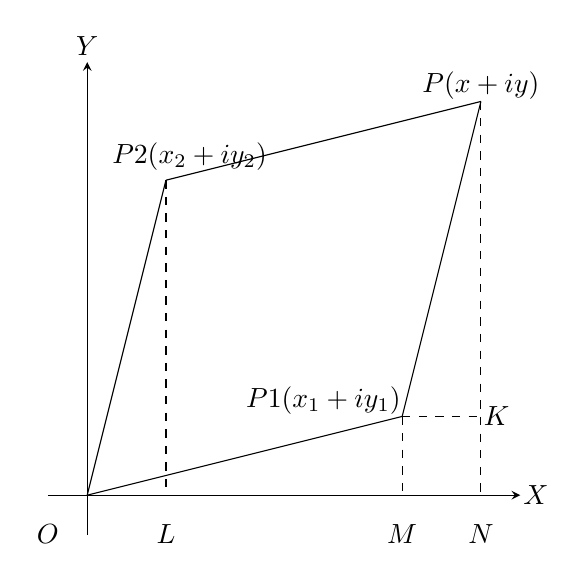
\begin{tikzpicture}
      \draw[->, >=stealth] (-.5,0) -- (5.5,0);
      \draw[->, >=stealth] (0,-.5) -- (0,5.5);
      \draw (5.7, 0) node {$X$};
      \draw (0,5.7) node {$Y$};
      \draw (0,0) -- (4,1);
      \draw (0,0) -- (1,4);
      \draw (1,4) -- (5,5);
      \draw (4,1) -- (5,5);
      \draw[dashed] (4,1) -- (4,0);
      \draw[dashed] (1,4) -- (1,0);
      \draw[dashed] (5,5) -- (5,0);
      \draw[dashed] (4,1) -- (5,1);
      \draw (-.5,-.5) node {$O$};
      \draw (1,-.5) node {$L$};
      \draw (4,-.5) node {$M$};
      \draw (5,-.5) node {$N$};
      \draw (5.2,1) node {$K$};
      \draw (3, 1.2) node {$P1(x_1+iy_1)$};
      \draw (1.3, 4.3) node {$P2(x_2+iy_2)$};
      \draw (5, 5.2) node {$P(x+iy)$};
    \end{tikzpicture}
    \caption{Complex numbers addition}
  \end{center}
\end{figure}
Clearly, $z = z_1 + z_2 = x_1 + x_2 + i(y_1 + y_2)$. Let $P_1M, P_2L$ and $PN$ be parallel to the $y$-axis; $P_1K$ be parallet to
the $x$-axis. This implied that triangle $OP_2L$ and $PP_1K$ are congruent.

We have $P_1K = OL = x_1$ and $P_2L = PK = y_1$

Thus, $ON = OM + MN = OL + P_1K = x_1 + x_2$ and $PN = PK + KN = P_2L + P_1M = y_2 + y_1$

So we can say that coordinates of $P$ are $(x_1 + x_2, y_1 + y_2)$ which represents the complex number $z.$

We also see that this obeys vector addition i.e. $OP_1 + OP_2 = OP_1 + P_1P = OP$

\subsection{Subtraction}
\begin{figure}[h]
  \begin{center}
    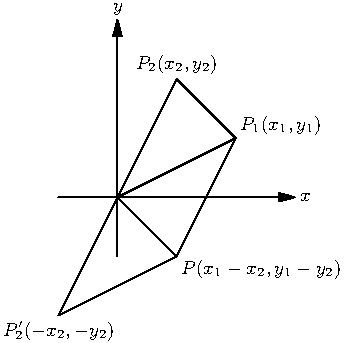
\includegraphics{complex-numbers-subtraction}
    \caption{Complex numbers subtraction}
    \label{fig:cns}
  \end{center}
\end{figure}
In figure \ref{fig:cns}, we first represent $-z_2$ by $P_2'$ so that  $P_2P_2'$ is bisected at $O.$ Complete the parallelogram $OP_1PP_2'.$ Then it can be
easily seen that $P$  representd the difference $z_1 - z_2.$

As $OP_1PP_2'$ is a parallelogram so $P_1P = OP_2'.$ Using vetor notation, we have, $z_1 - z_2 = OP_1 - OP_2 = OP_1 + OP_2' = OP_1 + P_1P = P_2P1$

It follows that the complex number $z_1 - z_2$ is represented by the vector $P_1P_2,$ where points $P_1$ and $P_2$ represent the
complex numbers $z_1$ and $z_2$ respectively.

It should be noted that $\arg(z_1 - z_2)$ is the angle through which $OX$ must be rotated in the anticlockwise direction to make it
parallel with $P_1P_2.$

\subsection{Multiplication}
\begin{figure}[H]
  \begin{center}
    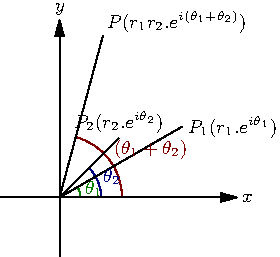
\includegraphics{complex-numbers-multiplication}
    \caption{Complex numbers multiplication}
  \end{center}
\end{figure}
For multiplication it is convenient to use Euler's formula of complex numbers.

Let $z_1 = r_1e^{i\theta_1}$ and $z_2 = r_2e^{i\theta_2},$ then clealry, $z_1z_2 = r_1r_2e^{i(\theta_1 + \theta_2)}$

\subsection{Division}
\begin{figure}[!h]
  \begin{center}
    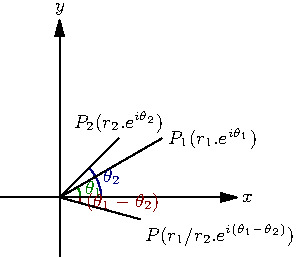
\includegraphics{complex-numbers-division}
    \caption{Complex numbers division}
  \end{center}
\end{figure}
For division also it is convenient to use Euler's formula of complex numbers.\\

Let $z_1 = r_1e^{i\theta_1}$ and $z_2 = r_2e^{i\theta_2},$ then clealry, $z_1/z_2 = r_1/r_2e^{i(\theta_1 - \theta_2)}$

\section{Three Important Results}
\begin{figure}[!h]
  \begin{center}
    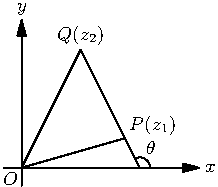
\includegraphics{complex-numbers-external-angle}
    \caption{External angle}
  \end{center}
\end{figure}
$z_1 - z_2 = \overrightarrow{OP} - \overrightarrow{OQ} = \overrightarrow{QP}$

$\therefore |z_1 - z_2| = |\overrightarrow{QP}| = QP$ which is nothing but distance between $P$ and $Q.$

$\arg(z_1 - z_2)$ is the angle made by $\overrightarrow{QP}$ with $x$-axis whis is nothing but $\theta.$
\begin{figure}[h]
  \begin{center}
    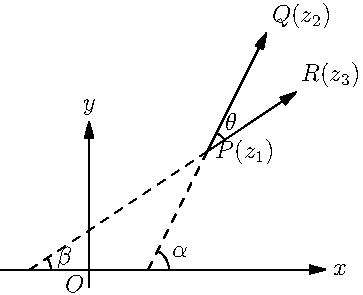
\includegraphics{angle-three-complex-numbers}
    \caption{Angle relation between three complex numbers}
    \label{fig:arbtcn}
  \end{center}
\end{figure}

In figure \ref{fig:arbtcn}, $\theta = \alpha - \beta = \arg(z_3 - z_1) - \arg(z_2 - z_1) \Rightarrow \theta = arg\frac{z_3 - z_1}{z_2 - z_1}$

Similarly if three complex numbers are vertices of a triangle then angles of those vertices can also be computed using previous
results.

Similarly, for four points to be concyclic where those points are represented by $z_1, z_2, z_3$ and $z_4$ if
$$arg\left(\frac{z_2 - z_4}{z_1 - z_4}.\frac{z_1 - z_3}{z_2 - z_4}\right) = 0$$

\section{More Roots}
\subsection{Any Root of an Complex Number is a Complex Number}
Let $x + iy$ be a complex number, where $y \neq 0$.

Let $(x +iy)^n = a\therefore x + iy = a^n$

Now, if $a$ is real, $a^n$ will also be real but from above a complex number $x + iy$ is equal to a real number, $a^n$, which is
not possible. Hence, it must be complex.

\subsection{Square Root of a Complex Number}
Consider a complex number $z = x + iy$. Let $a + ib$ be its square root. Then
$$\sqrt{x + iy} = a + ib \Rightarrow x + iy = (a^2 - b^2) + 2abi$$
Equating real and imaginary parts
$$x = a^2 - b^2, y = 2ab \Rightarrow (a^2 + b^2)^2 = (a^2 - b^2)^2 + (2ab)^2$$
From these two equations, we have
$$a = \pm\sqrt{\frac{\sqrt{x^2 + y^2} + x}{2}}, b = \sqrt{\frac{\sqrt{x^2 - y^2} - x}{2}}$$
\subsection{Cube Roots of Unity}
Let $x = \sqrt[3]{1} \Rightarrow x^3 - 1 = 0$

$\Rightarrow (x - 1)(x^2 + x + 1 ) = 0$

So the three roots are $x = 1, \frac{-1 \pm \sqrt{3}}{2}$ i.e. $1, \frac{-1\pm \sqrt{3}i}{2}$.

It can be easily verified that if $\omega = \frac{-1 -\sqrt{3}i}{2}$, then $\omega^2 = \frac{-1 + \sqrt{3}i}{2}$, thus, three cube
roots are represented as $1, \omega$ and $\omega^2$. $\omega$ is the symbol used for representing cube root of unity.
\subsubsection{Important Identities}
Following identities can be proved easily. The proof is left as an exercise to the reader.
\begin{enumerate}
\item $x^2 + x + 1 = (x - \omega)(x - \omega^2)$
\item $x^2 - x + 1 = (x + \omega)(x + \omega^2)$
\item $x^2 + xy + y^2 = (x - y\omega)(x - y\omega^2)$
\item $x^2 - xy + y^2 = (x + y\omega)(x + y\omega^2)$
\item $x^3 + y^3 = (x + y)(x + y\omega)(x + y\omega^2)$
\item $x^3 - y^3 = (x - y)(x - y\omega)(x - y\omega^2)$
\item $x^2 + y^2 + z^2 - xy - yz - zx = (x + y\omega + z\omega^2)(x + y\omega^2 + z\omega) \text{~or~} (x\omega + y\omega^2 +
  z)(x\omega^2 + y\omega + z)
  \text{~or~}(x\omega + y + z\omega^2)(x\omega^2 + y + z\omega)$
\item $x^3 + y^3 + z^3 - 3xyz = (x + y + z)(x + y\omega + z\omega^2)(x+ y\omega^2 + z\omega)$
\end{enumerate}

\subsection{$n$th Root of Unity}
$1 = \cos0 + i\sin 0 \Rightarrow \sqrt[n]{1} = \sqrt[n]{\cos0 + i\sin0}$

\noindent $=\cos\frac{2k\pi}{n} + i\sin\frac{2k\pi}{n}, \text{~where~} k = 0, 1, 2, 3, 4, \ldots (n - 1)$

\noindent $= e^{\frac{2k\pi}{n}} = 1, e^{\frac{i2\pi}{n}}, e^{\frac{i4\pi}{n}}, \ldots, e^{\frac{i2(n - 1)\pi}{n}} = 1, \alpha, \alpha^2,
\ldots, \alpha^{n - 1}, \text{~where~}\alpha = e^{\frac{i2\pi}{n}}$

\noindent Similar to cube roots of unity it can be proven that $1 + \alpha + \alpha^2 + \ldots + \alpha^{n - 1} = 0$
and $1.\alpha.\alpha^2.\ldots\alpha^{n - 1} = (-1)^{n - 1}$

\section{De Moivre's Theoremm}
This theorem's proof uses mathematical induction, so read the chapter on it.

\noindent\textbf{Statement:} If $n$ is any integer then $(\cos\theta + i\sin\theta)^n = \cos n\theta + i\sin n\theta$.

\noindent\textbf{Proof: Case I.} When $n$ is $0$. Clearly, $(\cos\theta + i\sin\theta)^0 = 1$

\noindent\textbf{Case II.} When $n$ is a positive integer. Clearly is it true for $n = 1$

\noindent Let it is true for $n = m$. Then $(\cos\theta + i\sin\theta)^m = \cos m\theta + i\sin m\theta$

\noindent For $n = m + 1, (\cos\theta + i\sin\theta)^{m + 1} = (\cos m\theta + i\sin m\theta)(\cos\theta + i\sin\theta) = \cos(m + 1)\theta +
i\sin(m + 1)\theta$ [this result comes from trigonometry]

\noindent Thus, by mathematical induction we have proven the theorem for positive integers.

\noindent\textbf{Case III.} When $n$ is negative number. For $n = -1, (\cos\theta + i\sin\theta)^{-1} = \frac{1}{\cos\theta +
  i\sin\theta}$

\noindent $= \frac{\cos\theta - \i\sin\theta}{\cos^2\theta + \sin^2\theta} = \cos\theta - i\sin\theta$

\noindent Let it be true for $n = -m, (\cos\theta + i\sin\theta)^{-m} = \cos m\theta - i\sin m\theta$

\noindent For $n = -(m + 1), (\cos\theta + i\sin\theta)^{-(m + 1)} = \frac{\cos m\theta - i\sin m\theta}{\cos\theta + i\sin\theta}$

\noindent $= (\cos m\theta - i\sin m\theta)(\cos\theta - i\sin\theta) = \cos(m + 1)\theta + i\sin(m + 1)\theta$

Thus, it is proven for negative numbers as well. Proof for fractional powers is left as an exercise.

\section{Some Important Geometrical Results}
\subsection{Section Formula}
Let $z_1 = x_1 + iy_1, z_2 = x_2 + iy_2$ then $z = x + iy$, which divides the previous two points in the ratio m;nm;n can be given
by using the results from coordinate geometry as below:
$$x = \frac{mx_2 + nx_1}{m + n}, y = \frac{my_2 + ny_1}{m + n} \text{~and~}z = \frac{mz_2 + nz_1}{m + n}$$
Extending this section formula, we can say that if there is a point which is mid-point i.e. divides a line in two equal parts, then
$m = 1$ and $n = 1$ then $z$ is given by $\frac{1}{2}(z_1 + z_2)$.
\subsection{Distance Formula}
Distance between $A(z_1)$ and $B(z_2)$ is given by $AB = |z_1 - z_2|$.
\subsection{Equation of a Line}
The equation between two points $z_1$ and $z_2$ is given by the determinant
$$\begin{vmatrix}z&\overline{z}&1\\z_1&\overline{z_1}&1\\z_2&\overline{z_2}&1\end{vmatrix} = 0$$
or,
$$\frac{z - z_1}{\overline{z} - \overline{z_1}} = \frac{z_1 - z_2}{\overline{z_1} - \overline{z_2}}$$
The parametric form is given by $z = iz_1 + (1 - t)z_2$
\subsection{Collinear Points}
Three points $z_1, z_2$ and $z_3$ are collinear if and only if
$$\begin{vmatrix}z_1&\overline{z_1}&1\\z_2&\overline{z_2}&1\\z_3&\overline{z_3}&1\end{vmatrix} = 0$$
\subsection{Parallelogram}
Four complex numbers $A(z_1), B(z_2), C(z_3)$ and $D(z_4)$ represent the vertices of a parallelogram if $z_1 + z_3 = z_2 +
z_4$.This result comes from the fact that diagonals of a parallelogram bisect each other.
\begin{figure}[h]
  \begin{center}
    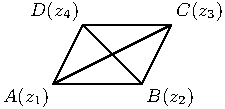
\includegraphics{complex-number-parallelogram}
    \caption{Parallelogram}
  \end{center}
\end{figure}
\subsection{Rhombus}
Four complex numbers $A(z_1), B(z_2), C(z_3)$ and $D(z_4)$ represent the vertices of a rhombus if $z_1 + z_3 = z_2 + z_4$ and
$|z_4 - z_1| = |z_2 - z_1|$.
\begin{figure}[h]
  \begin{center}
    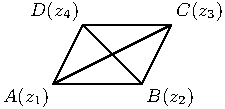
\includegraphics{complex-number-rhombus}
    \caption{Rhombus}
  \end{center}
\end{figure}
The diagonals must bisect each other. Thus, $z_1 + z_3 = z_2 + z_4.$ Also, four sides of a rhombus are equal i.e. $AD = AB
\Rightarrow |z_4 - z_1| = |z_2 - z_1|$.

\subsection{Square}
Four complex numbers $A(z_1), B(z_2), C(z_3)$ and $D(z_4)$ represent the vertices of a square if $z_1 + z_3 = z_2 + z_4,
|z_4 - z_1| = |z_2 - z_1|$ and $|z_3 - z_1| = |z_4 - z_2|$.
\begin{figure}[h]
  \begin{center}
    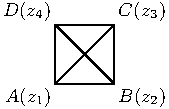
\includegraphics{complex-number-square}
    \caption{Square}
  \end{center}
\end{figure}

The diagonals must bisect each other. Thus, $z_1 + z_3 = z_2 + z_4.$ Also, four sides of a square are equal i.e. $AD = AB
\Rightarrow |z_4 - z_1| = |z_2 - z_1|$.

Also the digonals are equal in length so $|z_3 - z_1| = |z_4 - z_2|$.

\subsection{Rectangle}
Four complex numbers $A(z_1), B(z_2), C(z_3)$ and $D(z_4)$ represent the vertices of a square if $z_1 + z_3 = z_2 + z_4$ and $|z_3
- z_1| = |z_4 - z_2|$.
\begin{figure}[h]
  \begin{center}
    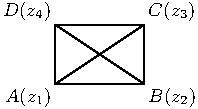
\includegraphics{complex-number-rectangle}
    \caption{Rectangle}
  \end{center}
\end{figure}

The diagonals must bisect each other. Thus, $z_1 + z_3 = z_2 + z_4$. Also, the digonals are equal in length so $|z_3 - z_1| = |z_4
- z_2|$.

\subsection{Centroid of a Triangle}
Let $A(z_1), B(z_2)$ and $C(z_3)$ be the vertices of a $\triangle ABC.$ Centroid $G(z)$ of the $\triangle ABC$ is the point of
concurrence of the medians of all three sides and is given by
$$z = \frac{z_1 + z_2 + z_3}{3}$$
\begin{figure}[h]
  \begin{center}
    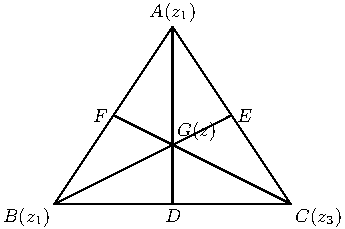
\includegraphics{complex-number-centroid}
    \caption{Centroid of a Triangle}
  \end{center}
\end{figure}

\subsection{Incenter of a Triangle}
Let $A(z_1), B(z_2)$ and $C(z_3)$ be the vertices of a $\triangle ABC.$ inceneter $I(z)$ of the $\triangle ABC$ is the point of
concurrence of the internal bisectors of and is given by
$$z = \frac{az_1 + bz_2 + cz_3}{a + b + c}$$
where $a, b, c$ are the lengths of the sides.

\subsection{Circumcenter of a Triangle}
Circumcenter $S(z)$ of a $\triangle ABC$ is the point of concurrence of perpendicular bisectors of sides of the triangle. It is
given by

$$z = \frac{(z_2 - z_3)|z_1|^2 + (z_3 - z_1)|z_2|^2 + (z_1 - z_2)|z_3|^2}{\overline{z_1}(z_2 - z_3) + \overline{z_2}(z_3 - z_1) + \overline{z_3}(z_1 - z_2)}$$
$$= \frac{\begin{vmatrix}|z_1|^2 & z_1 & 1\\ |z_2|^2 & z_2 & 1 \\ |z_3|^2 & z_3 & 1\end{vmatrix}}{\begin{vmatrix}\overline{z_1} & z_1 & 1\\\overline{z_2} & z_2 & 1\\\overline{z_3} & z_3 & 1 \end{vmatrix}}$$
Also,
$$z = \frac{z_1\sin2A + z_2\sin2B + z_3\sin2C}{\sin2A + \sin2B + \sin2C}$$

\subsection{Orthocenter of a Triangle}
The orthocenter $H(z)$ of the $\triangle ABC$ is the point of concurrence of altitudes of the side. It is given by
$$z = \frac{\begin{vmatrix}z_1^2 & \overline{z_1} & 1\\z_2^2 & \overline{z_2} & 1\\z_3^2 & \overline{z_3} & 1\end{vmatrix} + \begin{vmatrix}|z_1|^2 & z_1 & 1\\|z_2|^2 & z_2 & 1\\|z_3|^2 & z_3 & 1\end{vmatrix}}{\begin{vmatrix}\overline{z_1} & z_1 & 1\\\overline{z_2} & z_2 & 1\\\overline{z_3} & z_3 & 1\end{vmatrix}}$$
$$= \frac{z_1\tan A + z_2\tan B + z_3\tan C}{\tan A + \tan B + \tan C}$$
$$= \frac{z_1a\sec A + bz_2\sec B + cz_3\sec C}{a\sec A + b\sec B + c\sec C}$$

\subsection{Euler's Line}
The centroid $G$ of a triangle lies on the segment joining the orthocenter $H$ and the circumcenter $S$ of the triangle. $G$
divides the line $H$ and $S$ in the ratio $2:1$.

\subsection{Length of Perpendicular from a Point to a Line}
Length of a perpendicular of point $A(\omega)$ from the line $\overline{a}z + a\overline{z} + b = 0, (a\in C, b\in R)$
is given by

$$p = \frac{|\overline{a}\omega + a\overline{\omega} + b|}{2|a|}$$

\subsection{Equation of a Circle}
The equation of a circle with center $z_0$ and radius $r$ is $|z- z_0| = r$ or $z = z_0 + re^{i\theta}, 0\leq \theta\leq 2\pi$ or
$z\overline{z} - z_0\overline{z} - \overline{z_0}z + z_0\overline{z_0} - r^2 = 0$

\noindent General equation of a circle is $z\overline{z} - a\overline{z} + \overline{a}z + b = 0, (a\in C, b\in R)$ such that $\sqrt{a\overline{a} - b}\geq 0.$

\noindent Center of this circle is $-a$ and radius is $a\overline{a} - b.$

\noindent An equation of the circle, one of whose diameter is the line segment joining $z_1$ and $z_2$ is $(z - z_1)(\overline{z} - \overline{z_2}) + (\overline{z} - \overline{z_1})(z - z_2) = 0$

\noindent An equation of the the circle passing through two points $z_1$ and $z_2$ is
$$(z - z_1)(\overline{z} - \overline{z_2}) + (\overline{z} - \overline{z_1})(z - z_2) + k \begin{vmatrix}z & \overline{z} & 1\\z_1
  & \overline{z_1} & 1\\z_2 & \overline{z_2} & 1 \end{vmatrix} = 0$$
where $k$ is a parameter.

\subsection{Equation of a Circle Passing through Three Points}
\begin{figure}[h]
  \begin{center}
    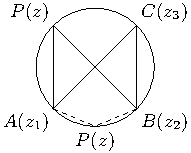
\includegraphics{complex-number-circle}
    \caption{Circle through three points}
  \end{center}
\end{figure}
We choose any point $P(z)$ on the circle. Two such points are shown in the figure above one is in same segment with $C$
and the other one in different segement. So we have
$$\angle ACB = \angle APB\text{~or~}\angle ACB + \angle APB = \pi$$
$$\arg\frac{z_3 - z_2}{z_3 - z_1} - arg\frac{z - z_2}{z - z_1} = 0\text{~or~}\arg\frac{z_3 - z_2}{z_3 - z_1} + arg\frac{z - z_2}{z - z_1} = \pi$$
Clearly, in both cases the fraction must be purely real. Thus we can apply the property of conjugates i.e. $z = \overline{z}$ which
also gives us the condition for four concyclic points.

$$\Rightarrow \frac{(z - z_1)(z_3 - z_2)}{(z - z_2)(z_3 - z_1)} = \frac{\overline{(z - z_1)(z_3 - z_2)}}{\overline{(z - z_2)(z_3 -
    z_1)}}$$
From this we can also deduce the condition for four points to be concyclic. Treating $P(z)$ as just another point $D(z_4)$, we can
rewrite the abobe result as
$$\frac{(z_4 - z_1)(z_3 - z_2)}{(z_4 - z_2)(z_3 - z_1)} = \frac{\overline{(z_4 - z_1)(z_3 - z_2)}}{\overline{(z_4 -
    z_2)(z_3 - z_1)}}$$

\subsection{Finding Loci by Examination}
\begin{enumerate}
\item $\\arg(z - z_0) = \alpha$

  If $\alpha$ is a real number and $z_0$ is a fixed point, then $\\arg(z - z_0) =\alpha$ represents a vector starting at
  $z_0$(exlcluding  the point $z_0$) and making an angle $\alpha$ with real $x$-axis.
  \begin{figure}[h]
    \begin{center}
      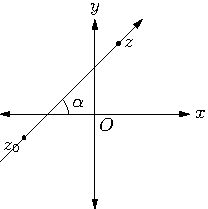
\includegraphics{complex-number-loci1}
    \end{center}
  \end{figure}

  Now suppose $z_0$ is origin $O$, then the above equation becomes $\\arg(z) = \alpha$, which is a vector starting at origin and
  making an angle $\alpha$, which is a vector starting at origin and making an angle $\alpha$ with $x$-axis.
\item If $z_1$ and $z_2$ are two fixed points such that $|z - z_1| = |z - z_2|$ then $z$ represents perpendicular bisector of the
  segment joining $A(z_1)$ and $B(z_2).$ And $z, z_1, z_2$ will form an isoscles triangle.
  \begin{figure}[h]
    \begin{center}
      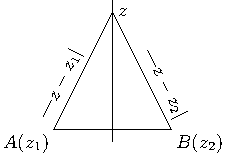
\includegraphics{complex-number-loci2}
    \end{center}
  \end{figure}

  If $z_1$ and $z_2$ are two fixed points and $k > 0, k\neq 1$ is a real number then $\frac{|z- z_1|}{|z - z_2|} = k$ represents a
  circle.
\item $|z - z_1| + |z - z_2| = k$. Let $z_1$ and $z_2$ be two fixed points and $k$ be a positive real number.
  \begin{enumerate}
    \item Refer figure \ref{fig:flbee}, if $k > |z - z_2|,$ then $|z - z_1| + |z - z_2| = k$ represents an ellipse with foci at $A(z_1)$ and $B(z_2)$ and length
      of major axis $= k$.
      \begin{figure}[h]
        \begin{center}
          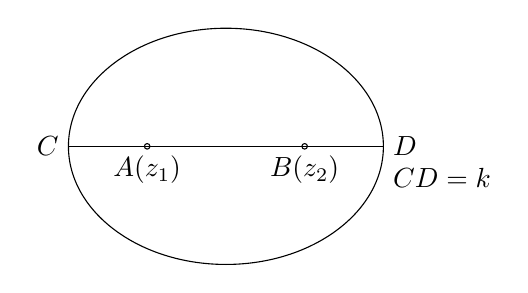
\begin{tikzpicture}
            \draw (0, 0) ellipse (2 and 1.5);
            \draw (-2, 0) node[anchor=east] {$C$} (2, 0) node[anchor=west] {$D$};
            \draw (-2, 0) -- (2, 0);
            \draw (-1, 0) node[anchor=north] {$A(z_1)$} (1, 0)
            node[anchor=north] {$B(z_2)$};
            \draw (-1, 0) circle(1pt) (1, 0) circle(1pt) (2, -.4)
            node[anchor=west] {$CD = k$};
          \end{tikzpicture}
          \caption{\label{fig:flbee}Locus of an Ellipse}
        \end{center}
      \end{figure}
    \item If $k = |z - z_2|$, then it represents the line segment joining $z_1$ and $z_2$.
    \item If $k < |z - z_2|$, thne it does not represent any curve/line in Argand plane.
  \end{enumerate}
\item If $|z - z_1| - |z - z_2| = k$. Let $z_1$ and $z_2$ be two fixed points and $k$ be a positive real number.
  \begin{enumerate}
  \item Refer figure \ref{fig:flbep}, if $k\neq |z - z_2|$, then it represnts a parabola with foci at $A(z_1)$ and $B(z_2)$.
    \begin{figure}[H]
      \begin{center}
        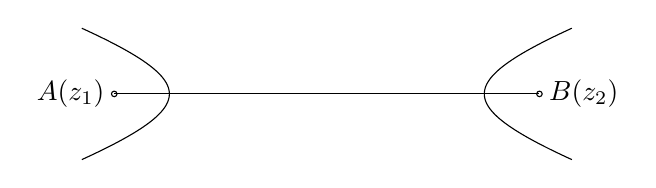
\begin{tikzpicture}
          \draw plot[variable=\t,samples=100,domain=-50:50]
          ({2*sec(\t)},{.7*tan(\t)});
          \draw plot[variable=\t,samples=100,domain=-50:50]
          ({-2*sec(\t)},{.7*tan(\t)});
          \draw (-2.7,0) -- (2.7, 0);
          \draw (-2.7, 0) circle(1pt) (2.7, 0) circle(1pt);
          \draw (-2.7, 0) node[anchor=east] {$A(z_1)$} (2.7, 0)
          node[anchor=west] {$B(z_2)$};
        \end{tikzpicture}
        \caption{\label{fig:flbep} Locus of a parabola}
      \end{center}
    \end{figure}
    \item If $k = |z_1 - z_2|$, then it represents the straight line joining $A(z_1)$ and $B(z_2)$ but excluding the segment $AB$
      \begin{figure}[H]
        \begin{center}
          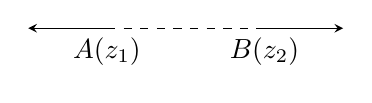
\begin{tikzpicture}
            \draw[dashed] (-1, 0) -- (1, 0);
            \draw[->, >= stealth] (-1, 0) -- (-2, 0);
            \draw[->, >= stealth] (1, 0) -- (2, 0);
            \draw (-1, 0) node[anchor=north] {$A(z_1)$} (1, 0) node[anchor=north] {$B(z_2)$};
          \end{tikzpicture}
        \end{center}
      \end{figure}
  \end{enumerate}
  \item $|z - z_1|^2 + |z - z_2|^2 = |z_1 - z_2|^2$. If $z_1$ and $z_2$ are two fixed points then it represents a circle with $z_1$
    and $z_2$ as the endpoints of one of the diameters.
    \begin{figure}[H]
      \begin{center}
        \begin{tikzpicture}
          \draw (0, 0) circle(2);
          \draw (-2, 0) -- (2, 0) (-2, 0) node[anchor=east] {$A(z_1)$}
          (2, 0) node[anchor=west] {$B(z_2)$};
          \draw (0, 0) circle(1pt) (0,0) node[anchor=north] {$O$};
        \end{tikzpicture}
      \end{center}
    \end{figure}
  \item $\arg\left(\frac{z - z_1}{z - z_2}\right) = \alpha$. Let $z_1$ and $z_2$ be any two fixed points and $\alpha$ be a real
    number such that $0\leq \alpha \leq \pi$.
    \begin{enumerate}
    \item If $0 < \alpha < \pi$ and $\alpha \neq \pi/2$, then it represents a segment of a circle passing through $A(z_1)$ and
      $B(z_2)$.
      \begin{figure}[H]
        \begin{center}
          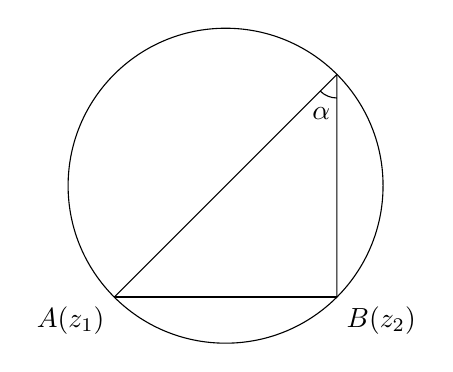
\begin{tikzpicture}
            \draw (0, 0) circle(2);
            \draw (-1.414, -1.414) -- (1.414, -1.414);
            \draw (-1.414, -1.414) -- (1.414, 1.414) (1.414, -1.414) -- (1.414,
            1.414);
            \draw (1.414, 1.114) arc(270:225:.3);
            \draw (-1.414, -1.414) node[anchor=north east] {$A(z_1)$} (1.414,
            -1.414) node[anchor=north west] {$B(z_2)$};
            \draw (1.214, 1.114) node[anchor=north] {$\alpha$};
          \end{tikzpicture}
        \end{center}
      \end{figure}
    \item If $\alpha = \pi/2$, then it represents a circle with diameter as the line segment joining $A(z_1)$ and $B(z_2)$.
      \begin{figure}[H]
        \begin{center}
          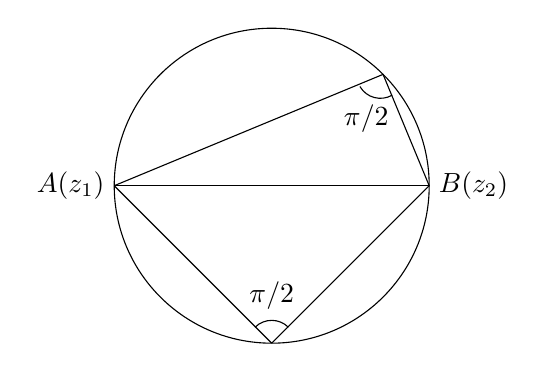
\begin{tikzpicture}
            \draw (0, 0) circle(2);
            \draw (-2, 0) -- (2, 0);
            \draw (-2, 0) -- (1.414, 1.414) (2, 0) -- (1.414, 1.414) (-2, 0) --
            (0, -2) (2, 0) -- (0, -2);
            \draw (-2, 0) node[anchor=east] {$A(z_1)$} (2,
            0) node[anchor=west] {$B(z_2)$};
            \draw (1.53, 1.15) arc(300:210:.3);
            \draw(.2121, -1.7979) arc(45:135:.3);
            \draw (1.2, 1.15) node[anchor=north] {$\pi/2$} (0, -1.7)
            node[anchor=south] {$\pi/2$};
          \end{tikzpicture}
        \end{center}
      \end{figure}
    \item If $\alpha = \pi$, then it represents the straight line joining $A(z_1)$ and $B(z_2)$ but excluding the line segment $AB$.
      \begin{figure}[H]
        \begin{center}
          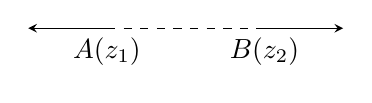
\begin{tikzpicture}
            \draw[dashed] (-1, 0) -- (1, 0);
            \draw[->, >= stealth] (-1, 0) -- (-2, 0);
            \draw[->, >= stealth] (1, 0) -- (2, 0);
            \draw (-1, 0) node[anchor=north] {$A(z_1)$} (1, 0) node[anchor=north] {$B(z_2)$};
          \end{tikzpicture}
        \end{center}
      \end{figure}
    \item If $\alpha = 0,$ then it represents the straight line joining $A(z_1)$ and $B(z_2)$.
      \begin{figure}[H]
        \begin{center}
          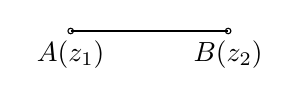
\begin{tikzpicture}
            \draw (-1, 0) -- (1, 0);
            \draw (-1, 0) node[anchor=north] {$A(z_1)$} (1, 0) node[anchor=north] {$B(z_2)$};
            \draw (-1, 0) circle(1pt) (1, 0) circle(1pt);
          \end{tikzpicture}
        \end{center}
      \end{figure}
    \end{enumerate}
\end{enumerate}

\section{Remainder Theorem}
If $f(x)$ us a polynomial in $x$ and if $f(a) = 0$, then $f(x)e$ is exactly divisible by $x - a$. Thus, we can say that an $n$th
degree polynomial can be resolved into $n$ equal or unequal factors. Let the polynomial $x^n + p_1x^{n - 1} + p_2x^{n - 2} + \ldots
+ p_{n - 1}x + p_n$ have the roots $x_1, x_2, \ldots, x_n$ so that there exists factorization $x^n + p_1x^{n - 1} + p_2x^{n - 2} + \ldots
+ p_{n - 1}x + p_n = (x - x_1)(x - x_2)\ldots(x - x_n)$.

We then have following relations:
$$x_1 + x_2 + \ldots + x_n = -p_1$$
$$x_1x_2 + x_1x_3 + \ldots + x_1x_n + x_2x_3 + \ldots + x_{n - 1}x_n = -p_2$$
$$x_1x_2x_3 + \ldots + x_{n -2}x_{n - 1}x_n = -p_3$$
$$\ldots$$
$$x_1x_2\ldots x_n = \pm p_n$$

\section{Problems}
Find the square root of the following complex numbers:

\begin{enumerate}
\item $7 + 8i$
\item $3 + 4i$
\item $a^2 - b^2 + 2abi$
\item $7 - 25\sqrt{-2}$
\item $\sqrt[4]{-81}$
\item Find the square root of $$\frac{x^2}{y^2} + \frac{y^2}{x^2} + \frac{1}{2i}\left(\frac{x}{y} + \frac{y}{x}\right) +
  \frac{31}{16}$$
\item Find the square root of $$\frac{x^2}{y^2} + \frac{y^2}{x^2} - \frac{1}{i}\left(\frac{x}{y} - \frac{y}{x}\right) -
  \frac{9}{4}$$
\item Find the square root of $$x^2 + \frac{1}{x^2} + 4i\left(x - \frac{1}{x}\right) - 6$$
\item Find $\sqrt{2 + 3\sqrt{-5}} + \sqrt{2 - 3\sqrt{-5}}$
\item Find $\sqrt{i}\sqrt{-i}$
\end{enumerate}

\noindent Simplify the following in the form of $A + iB$

\begin{enumerate}[resume]
\item $i^{n + 80} + i^{n + 50}$
\item $\left(i^{17} + \frac{1}{i^{15}}\right)^3$
\item $\frac{(1 + i)^2}{2 + 3i}$
\item $\left(\frac{1}{1 + i} + \frac{1}{1 - i}\right)\frac{7 + 8i}{7 - 8i}$
\item $\frac{(1 + i)^{4n + 7}}{(1 - i)^{4n - 1}}$
\item $\frac{1}{1 - \cos\theta + 2i\sin\theta}$
\item $\frac{(\cos x + i\sin x)(\cos y + i\sin y)}{(\cot u + i)(i + \tan v)}$
\item Evaluate i. $i^5$ ii. $i^{67}$ iii. $i^{-59}$ iv. $i^{2014}$
\item If $a<0, b>0$, then prove that $\sqrt{ab}$ is equal to $\sqrt{|a|b}i$.
\item Prove that $i^n + i^{n + 1} + i^{n + 2} + i^{n + 3} = 0$.
\item Find the value of the sum $\sum_{n = 1^13}(i^n + i^{n + 1})$
\item Simplify and find the value of $\frac{2^n}{(1 + i)^{2n}} + \frac{(1 + i)^{2n}}{2^n}$
\item Find different values of $i^n + i^{-n}, ~\forall~n\in I$.
\item If $4x + (3x - y)i = 3 - 6i$, then find the value of $x$ and $y$.
\item Find the value of $\left(\frac{1}{3} + i\frac{7}{3}\right) + \left(4 + i\frac{1}{3}\right) - \left(-\frac{4}{3} + i\right)$.
\item Find the real values of $x$ and $y$, if $\frac{(1 + i)x - 2i}{3 + i} + \frac{(2 - 3i)y + i}{3 - i} = i$.
\item Find the multiplicative inverse of $4 - 3i$.
\item If $z_1 = 2 + 3i$ and $z_2 = 1 + 2i$, then find the value of $z_1/z_2$.
\item If $z_1 = 9y^2 - 4 -i10x$ and $z_2 = 8y^2 -20i$ such that $z_1 = \overline{z_2}$, then find $z = x + iy$.
\item Find $z$ if $|z + 1| = z + 2(1 + i)$, where $z\in C$.
\item Find the modulus and argument of the complex number $\frac{1 + 2i}{1 - 3i}$
\item If $\frac{x - 3}{3 + i} + \frac{y - 3}{3 - i} = i$, where $x, y \in R$, then find $x$ and $y$.
\item What is the real part of $(1 + i)^{50}$.
\item If a complex number is $z$, such that $z + |z| = 2 + 8i$, then find $z$.
\item Find the sum of sequence $S = i + 2i^2 + 3i^3 + \ldots$ up to $100$ terms.
\item Find the value of the sum $\frac{1}{1 + i} + \frac{1}{1 - i} + \frac{1}{-1 + i} + \frac{1}{-1 -i} + \frac{2}{1 + i} +
  \frac{2}{1 - i} + \frac{2}{-1 + i} + \frac{2}{-1 -i} + \ldots + \frac{n}{1 + i} + \frac{n}{1 - i} + \frac{n}{-1 + i} +
  \frac{n}{-1 -i}$
\item Find the product of the real parts of the root $z^2 - z - 5 + 5i = 0$.
\item Find the number of complex numbers satisfying $z^3 + \overline{z} = 0$.
\item Find the number of real roots of the equation $z^3 + iz - 1= 0$.
\item In the following diagram, if given circle is unit circle then find the reciprocal of point $A.$
  \begin{figure}[H]
    \begin{center}
      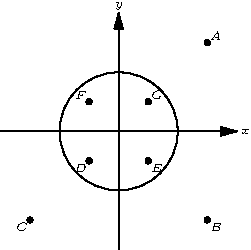
\includegraphics{complex-number-problem-40}
    \end{center}
  \end{figure}
\item If $z = (3 + 7i)(p + iq)$, where $p, q\in I$, is purely imaginary, then find the minimum value of $|z|^2$.
\item If $\alpha = \left(\frac{a - ib}{a + ib}\right)^2 + \left(\frac{a + ib}{a - ib}\right)^2,~\forall~a, b\in R$, then prove that
  $\alpha$ is real.
\item If $\beta = \frac{z - 1}{z + 1}$ such that $|z| = 1$, then prove that $\beta$ is imaginary.
\item If $|z - 3i| = 3$ such the $\arg(z)\in\left(0, \frac{\pi}{2}\right)$, then find the value of $\cos(\arg(z)) - \frac{6}{z}$.
\item Find the polar form of the complex number $\frac{-16}{1 + i\sqrt{3}}$
\item Let $z$ and $w$ be the two non-zero complex numbers such that $|z| = |w|$ and $\arg(z) + \arg(w) = \pi$, then prove that $z =
  -\overline{w}$.
\item If $x - iy = \sqrt{\frac{a - ib}{c - id}}$, then prove that $(x^2 + y^2)^2 = \frac{a^2 + b^2}{c^2 + d^2}$
\item Find the minimum value of $|z| + |z - 2|$.
\item If $|z_1 - 1|< 1, |z_2 - 2| < 2$ and $|z_3 - 3|< 3$, then prove that the maximum value of $|z_1 + z_2 + z_3|$ is $12$.
\item If $\alpha, \beta$ are two complex nnumbers, then prove that $|\alpha|^2 + |\beta|^2 = \frac{1}{2}(|\alpha + \beta|^2 +
  |\alpha - \beta|^2)$.
\item Show that for $z\in C, |z| = 0$, if and only if $z = 0$.
\item If $z_1$ and $z_2$ are $1 - i$ and $2 + 7i$, then find $Im\left(\frac{z_1z_2}{\overline{z_1}}\right)$.
\item If $|z - i|< 1$, then prove that $|z + 12 - 6i| < 14$.
\item If $|z + 6| = |2z + 3|$, then prove that $|z| = 3$.
\item If $\sqrt{a - ib} = x -iy$, then prove that $\sqrt{a + ib} = x + iy$.
\item If $x_r = \cos\frac{\pi}{2^r} + i\sin\frac{\pi}{2^2}$, then find the value of $x_1x_2x_3\ldots$ to $\infty$.
\item Find the value of $\frac{(\cos\theta + i\sin\theta)^4}{(\sin\theta + i\cos\theta)^2}$.
\item If $z = \left(\frac{\sqrt{3}}{2} + \frac{i}{2}\right)^5 + \left(\frac{\sqrt{3}}{2} - \frac{i}{2}\right)^5$, then find
  $\Im(z)$.
\item Find the product of all values of $\left(\cos\frac{\pi}{3} + i\sin\frac{\pi}{3}\right)^{\frac{3}{4}}$.
\item If $z_1$ and $z_2$ are two non-zero complex numbers such that$|z_1 + z_2| = |z_1| + |z_2|$, then find $\arg(z_1) - \arg(z_2)$.
\item If $z = 1 - \sin\alpha + i\cos\alpha$, where $\alpha \in \left(0, \frac{\pi}{2}\right)$, then find the modulus and principal
  value of the argument.
\item Find the value of expression $\left(\frac{1 + \sin\frac{\pi}{8} + i\cos\frac{\pi}{8}}{1 + \sin\frac{\pi}{8} -
  i\cos\frac{\pi}{8}}\right)^8$.
\item If $z_r = \cos\frac{2r\pi}{5} + i\sin\frac{2r\pi}{5}, r = 0, 1, 2, 3, 4$, then find $z_1z_2z_3z_4z_5$.
\item If $z_n = \cos\frac{\pi}{(2n + 1)(2n + 3)} + i\sin\frac{\pi}{(2n + 1)(2n + 3)}$, then find $z_1z_2z_3\ldots\infty$.
\item If $z_1, z_2$ be two complex numbers and $a, b$ are two real numbers, then prove that $|az_1 - bz_2|^2 + |bz_1 + az_2|^2 =
  (a^2 + b^2)(|z_1|^2 + |z_2|^2)$.
\item Show that the equation $\frac{A^2}{x - a} + \frac{B^2}{x - b} + \ldots + \frac{H^2}{x - h} = x + l$, where $A, B, \ldots H,
  a, b, \ldots, h$ and $l$ are real, cannot have imaginary roots.
\item Find all real number $x$, such that $|1 + 4i - 2^{-x}|\leq 5$.
\item Show that a unimodular complex number, not purely real can be expressed as $\frac{c + i}{c - i}$ for some real $c$.
\item If $(z^2 + 3)^2 = -16$, then find $|z|$.
\item If $\frac{\sin\frac{x}{2} + \cos\frac{x}{2} - i\tan x}{1 + 2i\sin\frac{x}{2}}$ is real, then find the set of all possible
  values of $x$.
\item Prove that $|z_1 + z_2|^2 + |z_1 - z_2|^2 = 2(|z_1|^2 + |z_2|^2)$.
\item If $x^2 - x + 1 = 0$, then find the value of $\sum_{n = 1}^5\left(x^n + \frac{1}{x^n}\right)^5$.
\item If $3^{49}(x + iy) = \left(\frac{3}{2} + \frac{\sqrt{3}}{2}i\right)^{100}$, then find $x$ and $y$.
\item For any two complex numbers $z_1$ and $z_2$, prove that $|z_1 + z_2|^2 = |z_1|^2 + |z_2|^2 + 2\Re(z_1\overline{z_2}) = |z_1|^2
  + |z_2|^2 + 2\Re(\overline{z_1}z_2)$.
\item If $|z_1| = |z_2| = 1$, then prove that $|z_1 + z_2| = \left|\frac{1}{z_1} + \frac{1}{z_2}\right|$.
\item If $|z - 2| = 2|z - 1|$, then prove that $|z|^2 = \frac{4}{3}\Re(z)$.
\item If $\sqrt[3]{a + ib} = x + iy$, then prove that $\frac{a}{x} + \frac{b}{y} = 4(x^2 - y^2)$.
\item If $x + iy = \sqrt{\frac{a + ib}{c + id}}$, then prove that $(x^2 + y^2)^2 = \frac{a^2 + b^2}{c^2 + d^2}$
\item If $z_1, z_2, \ldots, z_n$ are cube roots of unity, then prove that $|z_k| = |z_{k + 1}|~\forall~k\in[1, n - 1]$.
\item If $n$ is a positive integer greater than unity and $z$ is a complex number satisfying the equation $z^n = (1 + z)^2$, then
  prove that $\Re(z) < 0$.
\item Prove that $x^{3m} + x^{3n - 1} + x^{3r - 2}~\forall~m,n,r\in N$, is divisible by $1 + x + x^2$.
\item If $(\sqrt{3} + i)^n = (\sqrt{3} - i)^n~\forall~n\in N$, then prove that minimum value of $n$ is $6$.
\item If $(\sqrt{3} - i)^n = 2^n, n\in I$, the set of integers, then prove that $n$ is multiple of $12$.
\item If $z^4 + z^3 + 2z^2 + z + 1 = 0$, then prove that $|z| = 1$.
\item If $z = \sqrt[7]{-1}$, then find the value of $z^{86} + z^{175} + z^{289}$.
\item If $z^3 + 2z^2 + 3z + 2 = 0$, then find all the non-real, complex roots of the equation.
\item If $z$ is a non-real root of $z = \sqrt[5]{1}$, then find the value of $2^{|1 + z + z^2 + z^{-2} + z^{-1}|}$.
\item If $z$ is a non-real root of unity, then find the value of $1 + 3z + 5z^2 + \ldots + (2n - 1)z^{n - 1}$.
\item Find the value of $\sqrt{-1 - \sqrt{-1 - \sqrt{-1 - \text{~to~} \infty}}}$.
\item If $z = e^{\frac{i2\pi}{n}}$, then find the value of $(11 - z)(11 - z^2)\ldots(11 - z^{n - 1})$.
\item If $\frac{3}{2 + \cos\theta + i\sin\theta} = a + ib$, then prove that $a^2 + b^2 = 4a - 3$.
\item If $|2z - 1| = |z - 2|$, then prove that $|z| = 1$.
\item If $x$ is real and $\frac{1 - ix}{1 + ix} = m + in$, then prove that $m^2 + n^2 = 1$.
\item Find the general equation of the straigt line joining the points $z_1 = 1 + i$ and $z_2 = 1 - i$.
\item If $z_1, z_2, z_3$ are three complex numbers such that $5z_1 - 13z_2 + 8z_3 = 0$, then prove that $$\begin{vmatrix}z_1 &
  \overline{z_1} & 1\\ z_2 & \overline{z_2} & 1\\ z_3 & \overline{z_3} & 1\end{vmatrix} = 0$$
\item Find the length of perpendicualr from $P(2 - 3i)$ to the line $(3 + 4i)z + (3 - 4i)\overline{z} + 9 = 0$.
\item If a point $z_1$ is a reflection of a point $z_2$ through the line $z\overline{z} + \overline{b}z = c, b\neq 0$ in the argand
  plane, thne prove that $\overline{b}z_2 + b\overline{z_1} = c$.
\item The point represented by the complex number $2 - i$ is rotated by origin by an angle $\pi/2$ in the anti-clockwise
  direction. Find the new coordinates.
\item A particle $P$ starts from the point $z_0 = 1 + 2i$. It first moves horizontally, away from origin by $5$ units and then
  vertically, away from origin by $3$ units to reach a point $z_1$. From $z_1$ the particle moves $\sqrt{2}$ units in the
  direction of vector $\hat{i} + \hat{j}$ and it then rotaes about origin in anti-clockwise direction for an angle $\pi/2$
  to reach $z_2.$ Find the coordinates of $z_2$.
\item A man walks a distance of $3$ units from the origin in North-East direction. Then he walks $4$ units in North-West
  direction. Find the final coordinates.
\item If three complex numbers satisfty the relationship $\frac{z_1 - z_3}{z_2 - z_3} = \frac{1 - i\sqrt{3}}{2}$, then
  prove that $z_1, z_2$ and $z_3$ form an equilateral triangle.
\item If $z_1, z_2$ and $z_3$ form an equilateral triangle then prove that $z_1^2 + z_2^2 + z_3^2 = z_1z_2 + z_2z_3
  +z_3z_1$, and hence $\frac{1}{z_1 - z_2} + \frac{1}{z_2 - z_3} + \frac{1}{z_3 - z_1} = 0$.
\item If $z_1, z_2$ and $z_3$ are vertices of an equilateral triangle and $z_0$ is the circumcenter then prove that
  $3z_0^2 = z_1^2 + z_2^2 + z_3^2.$
\item If $z_1, z_2$ and $z_3$ form a right-angled, isosceles triangle with right angle at $z_3,$ then prove that $(z_1 -
  z_2)^2 = 2(z_1 - z_3)(z_3 - z_2)$.
\item Find the equation of the circle whose center is $z_0$ and radius is $r$.
\item If $z = 1 - t + i\sqrt{t^2 + t + 2},$ where $t$ is a real parameter. Prove that locus of $z$ in argand plane is a
  hyperbola.
\item Find the locus of $z$ if $\overline{z} = \overline{a} + \frac{r^2}{z - a}$.
\item If the equation $|z - z_1|^2 + |z - z_2|^2 = k$ represents the equation of a cirlce, where $z_1 = 2 + 3i, z_2 = 4 +
  3i$ are the ends of a diameter, then find the value of $k$.
\item If $|z + 1| = \sqrt{2}|z - 1|,$ then show that locus of $z$ is a circle.
\item Prove that the locus of $z$ given by $\left|\frac{z - 1}{z - i}\right| = 1$ is a straight line.
\item Find the condition for four complex numbers $z_1, z_2, z_3$ and $z_4$ to lie on a cyclic quadrilateral.
\item If $z_1, z_2$ and $z_3$ are complex numbers, such that $\frac{2}{z_1} = \frac{1}{z_2} + \frac{1}{z_3},$ then show
  that these points lie on a circle passing through origin.
\item If $|z - \omega|^2 + |z - \omega^2|^2 = r^2,$ where $r$ is radius and $\omega, \omega^2$ are cube roots of unity
  and ends of diameter of the circle then find radius.
\item Find the region represented by $|z - 4| < |z - 2|$.
\item If $2z_1 - 3z_2 + z_3 = 0$, then find the geometrical relationship between them.
\item If $z = x + iy,$ such that $|z + 1| = |z - 1|$ and $\arg\frac{z - 1}{z + 1} = \frac{\pi}{4},$ find $x$ and $y$.
\item If $|z|^8 = |z - 1|^8,$ then prove that roots of this equation are collinear.
\item Prove that $z\overline{z} + a\overline{z} + \overline{a}z + b = 0,$ represents a circle if $|a|^2 > b$.
\item If $z = (\lambda + 3) + i\sqrt{3 - \lambda^2},$ where $|\lambda| < \sqrt{3},$ then prove that it represents a circle.
\item If $z$ is a complex number such that $|\Re(z)| + |\Im(z)| = k,~\forall~ k\in R,$ then find the locus of $z$.
\item Consider a sequence of complex numbers such that $z_{n + 1} = z_n^2 + i,~\forall n\geq 1,$ where $z_1 = 0.$ Find $z_{111}$.
\item The complex numbers whose real and imaginary parts are integers and satisfy the relation $z\overline{z}^3 +
  z^3\overline{z} = 350,$ forms a rectangle in the argand plane. Find length of its diagonals.
\item If $z_1, z_2$ are two complex numbers and $\arg\frac{z_1 + z_2}{z_1 - z_2}$ but $|z_1 + z_2|\neq |z_1 - z_2|$ then
  find the figure formed by $0, z_1, z_2$ and $z_1 + z_2.$
\item If $z_1$ and $z_2$ are complex numbers such that $a|z_1| = b|z_2|, a, b\in R,$ then prove that $\frac{az_1}{bz_2} +
  \frac{bz_2}{az_1}$ lies on the segment $[-2, 2]$ of the real axis.
\item If $z_1, z_2, z_3$ are roots of the equation $z^3 + 3\alpha z^2 + 3\beta z + \gamma = 0,$ such that they form an
  equilateral triangle then prove that $\alpha^2 = \beta$.
\item If $z_1^2 + z_2^2 + 2z_1z_2\cos\theta = 0,$ then prove that $z_1, z_1$ and the origin form an isosceles triangle.
\item $A, B$ and $C$ represent $z_1, z_2$ and $z_3$ on argnad plane. The circumcenter of this triangle lies on the
  origin. If the altitude $AD$ meets circumcircle again at $P,$ then find the complex number representing $P$.
\item If $z_1$ and $z_2$ are the roots of the equation $z^2 + pz + q = 0,$ where $p,q$ can be complex numbers. Let $A, B$
  represent $z_1, z_2$ in the complex plane. If $\angle AOB = \alpha \neq 0$ and $OA = OB,$ where $O$ is the origin then find
  $p^2$.
\item If $Re\left(\frac{z + 4}{2x - 1}\right) = \frac{1}{2}$ then prove that locus of $z$ is a straight line.
\item If $z_1, z_2$ and $z_3$ are vertices of an equilateral triangle inscribed in the circle $|z| = 2.$ If $z_1, z_2,
  z_3$ are in clockwise sense then find $z_2$ and $z_3$.
\item If $z_1 = \frac{a}{1 - i}, z_2 = \frac{b}{2 + i}, z_3 = a - bi$ for $a, b\in R$ and $z_1 - z_2 = 1.$ Then find the
  centroid of the triangle formed by $z_1, z_2$ and $z_3$.
\item Let $\lambda \in R$. If the origin and the non-real roots of $2z^2 + 2z + \lambda = 0$ form three vertices of an
  equilateral triangle in the argand plane, then find $\lambda.$
\item If $a, b, c$ and $u, v, w$ are complex numbers such that $c = (1 - r)a + rb$ and $w = (1 - r)u + rv,$ where $r$ is
  a complex number then prove that the triangles are similar.
\item Find the intercept made by the circle $z\overline{z} + \overline{\alpha}z + \alpha\overline{z} + r = 0$ on real
  axis on the complex plane.
\item If $a = \cos\alpha +i\sin\alpha, b = \cos\beta + i\sin\beta, c = \cos\gamma + i\sin\gamma$ and $\frac{a}{b} +
  \frac{b}{c} + \frac{c}{a} = 1,$ then find the value of $\cos(\alpha - \beta) + \cos(\beta - \gamma) + \cos(\gamma - \alpha)$.
\item Find the locus of the center of a circle which touches the circles $|z - z_1| = a$ and $|z - z_2| = b$ externally.
\item Prove that $\tan\left[i\log\left(\frac{a - ib}{a + ib}\right)\right] = \frac{2ab}{a^2 - b^2}$.
\item $z_1 = a + ib$ and $z_2 = c + id$ are complex numbers such that $|z_1| = |z_2| = 1$ and $\Re(z_1\overline{z_2}) =
  0.$ Also, $w_1 = a + ic, w_2 = b + id$ then prove that $|w_1| = |w_2| = 1$ and $\Re(w_1\overline{w_2}) = 0$.
\item If $\left|\frac{z_1}{z_2}\right| = 1$ and $\arg(z_1z_2) = 0,$ then prove that $|z_2|^2 = z_1z_2$.
\item Find the value of the expression $2\left(1 + \frac{1}{\omega}\right)\left(1 + \frac{1}{\omega^2}\right) + 3\left(2
  + \frac{1}{\omega}\right)\left(2 + \frac{1}{\omega^2}\right) + 4\left(3 + \frac{1}{\omega}\right) \left(3 +
  \frac{1}{\omega^2}\right) + \ldots + (n + 1)\left(n + \frac{1}{\omega}\right)\left(n + \frac{1}{\omega^2}\right)$.
\item If $z_1$ and $z_2$ are two complex numbers satisfying the equation $\left|\frac{z_1 + iz_2}{z_1 -
  iz_2}\right| = 1$, then prove that $\frac{z_1}{z_2}$ is purely real.
\item If $z = -2 + 2\sqrt{3}i,$ then find values of $z^{2n} + 2^{2n}z^n + 2^{4n}$.
\item If $2\cos\theta = x + \frac{1}{x}$ and $2\cos\phi = y + \frac{1}{y},$ then find the values of $\frac{x}{y} +
  \frac{y}{x}, xy + \frac{1}{xy}$.
\item The complex numbers $z_1$ and $z_2$ such that $z_1\neq z_2$ and $|z_1| = |z_2|$. If $z_1$ has positive real part
  and $z_2$ has negative imaginary part, prove that $\frac{z_1 + z_2}{z_1 - z_2}$ is purely imaginary.
\item If $A(z_1), B(z_1)$ and $C(z_3)$ are the vertices of a $\triangle ABC$ in which $\angle ABC = \frac{\pi}{4}$ and
  $\frac{AB}{BC} = \sqrt{2},$ then prove that the value of $z_2 = z_3 + i(z_1 - z_3)$.
\item If $z_1z_2\in C, z_1^2 + z_2^2 \in R, z_1(z_1^2 - 3z_2^2) = 2$ and $z_2(3z_1^2 - z_2^2) = 11$, then find the value
  of $z_1^2 + z_2^2$.
\item If $\sqrt{1 - c^2} = nc - 1$ and $z = e^{i\theta}$, then find the value of $\frac{c}{2n}(1 + nz)\left(1 +
  \frac{n}{z}\right)$.
\item Consider an eclipse having its foci at $A(z_1)$ and $B(z_2)$ in the argand plane. If the eccentricity of the
  ellipse is $e$ and it is known that origin is an interior point of the ellipse, then prove that $e\in \left(0, \frac{|z_1 -
    z_2|}{|z_1| + |z_2|}\right)$
\item If $|z - 2 -i| = |z|\left|\sin\left(\frac{\pi}{4} - \arg(z)\right)\right|$, then find the locus of $z$.
\item Find the maximum area of the triangle formed by the complex coordinates $z z_1$ and $z_2$, which satisfy the
  relation $|z - z_1| = |z - z_2|$ and $\left|z - \frac{z_1 + z_2}{2}\right|\leq r$, where $r > |z_1 - z_2|$.
\item If $z_1 = a_1 + ib_1$ and $z_2 = a_2 + ib_2$ are complex numbers such that $|z_1| = 1, |z_1| = 2$ and $\Re(z_1z_2) =
  0,$ and $\omega_1 = a_1 + \frac{ia_2}{2}$ and $\omega_2 = 2b_1 + ib_2$, then prove that $|\omega_1| = 1, |\omega_2| = 2$ and
  $\Re(\omega_1\omega_2) = 0$.
\item Let $z$ be a complex number and $a$ be $a$ be a real number such that $z^2 + az + a^2 = 0,$ then prove that i)
  locus of $z$ is a pair of straight lines ii) $\arg(z) = \pm\frac{2\pi}{3}$ iii) $|z| = |a|$
\item If $x + \frac{1}{x} = 1$ and $p = x^{4000} + \frac{1}{x^{4000}}$ and $q$ is the the digit at units place in
  $2^{2^n} + 1, n\in N$ and $n > 1$, then find $p + q$.
\item Consider an equilateral triangle $A\left(\frac{2}{\sqrt{3}}e^{i\pi/2}\right),
  B\left(\frac{2}{\sqrt{3}}e^{-i\pi/6}\right)$ and $C\left(\frac{2}{\sqrt{3}}e^{-i5\pi/6}\right)$. If $P(z)$ is any point on the
  incircle then find the value of $AP^2 + BP^2 + CP^2$.
\item If $A_1, A_2, \ldots, A_n$ be the vertices of a regular polygon of $n$ sides in a circle of unit radius and $a =
  |A_1A_2|^2 + |A_1A_3|^2 + \ldots + |A_1A_n|^2, b = |A_1A_2||A_1A_3|\ldots |A_1A_n|$, then find $\frac{a}{b}$.
\item If $\left(1 + i\frac{x}{a}\right)\left(1+ i\frac{x}{b}\right)\left(1 + i\frac{x}{c}\right)\ldots = A + iB$, then
  prove that $\left(1 + \frac{x^2}{a^2}\right)\left(1 + \frac{x^2}{b^2}\right)$
  $\left(1 + \frac{x^2}{c^2}\right) \ldots = A^2 + B^2$.
\item Find the range of real number $\alpha$ for which the equations $z+\alpha|z-1|+2i=0;z=x+iy$ has a solution. Also,
  find the solution.
\item For every real number $a\geq0$, find all the complex numbers satisfying the equation $2|z| - 4az+1+ia=0$.
\item Show that $(x^2 + y^2)^5 = (x^5 - 10x^3y^2 + 5xy^4) + (5x^4y - 10x^2y^3 + y^5)^2$.
\item Express $(x^2+a^2)(x^2+b^2)(x^2+c^2)$ as sum of two squares.
\item If $(1 + x)^n = a_0 + a_1x + a_2x^2 + \ldots + a_nx^n$, then prove that $2^n = (a_0 - a_2 + a_4 - \ldots)^2 + (a_1
  - a_3 + a_5 - \ldots)^2$.
\item Dividing $f(z)$ by $z -i$, we get $i$ as remainder and if we divide by $z+i$, we get $1+i$ as remainder. Find the
  remainder upon division of $f(z)$ by $z^2+1$.
\item If $|z|\leq 1, |w|\leq 1,$ show that $|z - w|^2 \leq (|z| - |w|)^2 + [\arg(z) - \arg(w)]^2$.
\item If $z$ is any complex number, then show that $\left|\frac{z}{|z|} - 1\right| \leq |arg(z)|$.
\item If $z$ is any complex number, then show that $|z-1| \leq ||z|-1|+|z||argz|$.
\item If $\left|z + \frac{1}{z}\right| = a$, where $z$ is a complex number and $a > 0$, find the greatest and least
  values of $|z|$.
\item If $z_1, z_2$ be complex numebrs and $c$ is a positive number, prove that $|z_1 + z_2|^2 < (1 + c)|z_1|^2 + \left(1
  + \frac{1}{c}\right)|z_2|^2$.
\item If $z_1$ and $z_2$ are two complex numbers such that $\left|\frac{z_1 - z_2}{z_1 + z_2}\right| = 1$, prove that
  $\frac{iz_1}{z_2} = x$ where $x$ is a real number. Find the angle between the lines from origin to the points $z_1 + z_2$ and
  $z_1 - z_2$ in terms of $x$.
\item Let $z_1, z_2$ be any two complex numbers and $a, b$ be two real numbers such that $a^2 + b^2 \neq 0$. Prove that
  $|z_1|^2 + |z_2|^2 - |z_1^2 + z_2^2| \leq 2\frac{|az_1 + bz_2|^2}{a^2 + b^2}\leq |z_1|^2 + |z_2|^2 + |z_1^2 + z_2^2|$.
\item If $b + ic = (1 + a)z$ and $a^2 + b^2 + c^2 = 1$, prove that $\frac{a + ib}{1 + c} = \frac{1 + iz}{1 - iz}$, where
  $a, b,c$ are real numbers and $z$ is a complex number.
\item If $a, b, c, \ldots, k$ are all $n$ real roots of the equation $x^n + p_1x^{n - 1} + p_2x^{n - 2} + \ldots + p_{n -
  1}x + p_n = 0$, where $p_1, p_2, \ldots, p_n$ are real, show that $(1 + a^2)(1 + b^2)\ldots (1 + k^2) = (1 - p_2 + p_4 +
  \ldots)^2 + (p_1 - p_3 + \ldots)^2$.
\item If $f(x) = x^4 - 8x^3 + 4x^2 + 4x + 39$ and $f(3 + 2i) = a + ib$, find $a:b$.
\item Let $A$ and $B$ be two complex numbers such that $\frac{A}{B} + \frac{B}{A}= 1$, prove that the triangle formed by
  origin and these two points is equilateral.
\item If $n > 1$, show that the roots of the equation $z^n = (1 + z)^n$ are collinear.
\item If $A,B,C$ and $D$ are four complex number then show that $AD.BC\leq BD.CA + CD.AB$.
\item If $a, b\in R$ and $a, b\neq 0$, then show that the equation of line joining $a$ and $ib$ is $\left(\frac{1}{2a} -
  \frac{i}{2b}\right)z + \left(\frac{1}{2a} + \frac{i}{2b}\right)\overline{z} = 1$.
\item If $z_1$ and $z_2$ are two compelx numbers such that $|z_1| - |z_2| = |z_1 - z_2|$, then show that $\arg(z_1) -
  \arg(z_2) = 2n\pi$ where $n\in I$.
\item Let $A, B, C, D, E$ be points in the complex plane representing complex numbers $z_1, z_2, z_3, z_4, z_5$
  respectvely. If $(z_3 - z_2)z_4 = (z_1 - z_2)z_5,$ prove that $\triangle ABC$ and $\triangle DOE$ are similar.
\item Let $z$ and $z_0$ are two complex numbers and $z, z_0, z\overline{z_0}, 1$ are represented by points $P, P_0, Q, A$
  respectively. If $|z| = 1$, show that the triangle $POP_0$ and $AOQ$ are congruent and hence $|z - z_0| = |z\overline{z_0} - 1|$,
  where $O$ represents the origin.
\item If the line segment joining $z_1$ and $z_2$ is divided by $P$ and $Q$ in the ratio $a:b$ internally and externally,
  then find $OP^2 + OQ^2$ where $O$ is origin.
\item Let $z_1, z_2, z_3$ be three complex numbers and $a, b, c$ be real numbers not all zero such that $a + b + c = 0$
  and $az_1 + bz_2 + cz_3 = 0$, then show that $z_1, z_2, z_3$ are collinear.
\item If $z_1 + z_2 + \ldots + z_n = 0$, prove that if a line passes through origin then all these do not lie of the same
  side of the line provided they do not lie on the line.
\item The points $z_1 = 9 + 12i$ and $z_2 = 6 - 8i$ are given on a complex plane. Find the equation of the angle formed
  by the vector representing $z_1$ and $z_2$.
\item If the vertices of a $\triangle ABC$ are represented by $z_1, z_2, z_3$ respectively, then show that the
  orthocenter of $\triangle ABC$ is $\frac{z_1a\sec A + z_2b\sec B + z_3c\sec C}{a\sec A + b\sec B + c\sec C}$ or

  $\frac{z_1\tan A + z_2\tan B + z_3\tan C}{\tan A + \tan B + \tan C}$.
\item If the vertices of a $\triangle ABC$ are represented by $z_1, z_2$ and $z_3$ respectively, show that its
  circumcenter is $\frac{z_1\sin 2A + z_2\sin 2B + z_3\sin 2C}{\sin 2A + \sin 2B + \sin 2C}$.
\item If the vertices of a $\triangle ABC$ are represented by $z_1, z_2$ and $z_3$ respectively, show that its
  circumcenter is $\frac{z_1\sin 2A + z_2\sin 2B + z_3\sin 2C}{\sin 2A + \sin 2B + \sin 2C}$.
\item Find the orthocenter of the triangle with vertices $z_1, z_2, z_3$.
\item $ABCD$ is a rhombus described in clockwise direction. Suppose that the vertices $A, B, C, D$ are given by $z_1,
  z_2, z_3, z_4$ respectively and $\angle CBA = 2\pi/3$. Show that $2\sqrt{3}z_2 = (\sqrt{3} - i)z_1 + (\sqrt{3} + i)z_3$ and
  $2\sqrt{3}z_4 = (\sqrt{3} + i)z_1 + (\sqrt{3} - i)z_3$.
\item The points $P, Q$ and $R$ represent the numbers $z_1, z_2$ and $z_3$ respectively and the angles of the $\triangle
  PQR$ at $Q$ and $R$ are both $\frac{1}{2}(\pi - \alpha)$. Prove that $(z_3 - z_2)^2 = 4(z_3 - z_1)(z_1 -
  z_2)\sin^2\frac{\alpha}{2}$.
\item Points $z_1$ and $z_2$ are adjacent vertices of a regular polygon of $n$ sides. Find the vertex $z_3$ adjacent to
  $z_2(z_1\neq z_3)$.
\item Let $A_1, A_2, \ldots, A_n$ be the vertices of an $n$ sided regular polygon such that $\frac{1}{A_1A_2} =
  \frac{1}{A_1A_3} + \frac{1}{A_1A_4}$, find the value of $n$.
\item If $|z| = 2$, then show that the points representing the complex numbers $-1 + 5z$ lie on a circle.
\item If $|z - 4 + 3i|\leq 2,$ find the least and tghe greatest values of $|z|$ and hence find the limits between which
  $|z|$ lies.
\item If $z - 6 - 8i\leq 4$, then find the least and greatest value of $z$.
\item If $z - 25i\leq 15$ then find the least positive value of $\arg(z)$.
\item Show that the equation $|z - z_1|^2 + |z - z_2|^2 = k$ where $k\in R$ will represent a circle if $k\geq \frac{1}{2}|z_1 -
  z_2|^2$.
\item If $|z - 1| = 1$, prove that $\frac{z - 2}{z} = i\tan(\arg z)$.
\item Find the locus of $z$ if $\arg\left(\frac{z - 1}{z + 1}\right) = \frac{\pi}{4}$
\item If $\alpha$ is real and $z$ is a complex number and $u$ and $v$ be the real and imaginary parts of $(z - 1)(\cos\alpha -
  i\sin\alpha) + (z - 1)^{-1}(\cos\alpha + i\sin\alpha)$, prove that the locus of points representing the complex number such that
  $v =0$ is a circle of unit radius with center at point $(1, 0)$ and a straight line through the center of the circle.
\item If $|a_n| < 2$ for $n = 1, 2, 3, \ldots$ and $1 + a_1z + a_2z^2 + \ldots + a_nz^n = 0$, show that $z$ does not lie in the
  interior of the circle $|z| = \frac{1}{3}$.
\item Show that the roots of the equation $z^n\cos\theta_0 + z^{n - 1}\cos\theta_1 + \ldots + \cos\theta_n = 2$, where $\theta_1 +
  \theta_2 + \ldots + \theta_n\in R$ lies outside the circle $|z| = \frac{1}{2}$.
\item $z_1, z_2, z_3$ are non-zero, non-collinear complex numbers such that $\frac{2}{z_1} = \frac{1}{z_2} + \frac{1}{z_3}$, show
  that $z_1, z_2, z_3$ lie on a circle passing through origin.
\item $A, B, C$ are the points representing the complex numbers $z_1,z_2,z_3$ respectively on the complex plane and the
  circumcenter of the $\triangle ABC$ lies on the origin. If the altitude of the triangle through the vertex $A$ meets the circle
  again at $P$, prove that $P$ represents the complex number $\frac{z_2z_3}{z_1}$.
\item Two different non-parallel lines cuut the circle $|z| = r$ at points $a, b, c, d$ respectively. Prove that these two lines
  meet at a point given by $\frac{a^{-1} + b^{-1} + c^{-1} + d^{-1}}{a^{-1}b^{-1}c^{-1}d^{-1}}$.
\item Let $z_1, z_2, z_3$ be three non-zero complex numbners such that $z_2\neq 1, a = |z_1|, b = |z_2|$ and $c =
  |z_3|$. If $$\begin{vmatrix} a & b & c\\ b & c & a\\ c & a & b\end{vmatrix} = 0$$

    then show that $\arg\left(\frac{z_3}{z_2}\right) = \arg\left(\frac{z_3 - z_1}{z_2 - z_1}\right)^2$
\item $P$ is a point on a circle wit $OP$ as diameter. Two points $Q$ and $R$ are taken such that $\angle POQ = \angle QOR =
  \theta$. If $O$ is the origin and $P, Q$ and $R$ are represented by the complex numbers $z_1, z_2$ and $z_3$ respectively, show
  that $z_2^2\cos2\theta = z_1z_3\cos^2\theta$.
\item Find the equation in complex variables of all circles which are orthogonal to $|z| = 1$ and $|z - 1| = 4$.
\item Find the real values of the parameter $t$ for which there is at least one complex number $z = x + iy$ satisfying the
  condition $|z + 3| = t^2 - 2i + 6$ and the ineuqality $z - 3\sqrt{3}i < t^2$.
\item If $a, b, c$ and $d$ are real and $ad > bc$, show that the imaginary parts of the complex number $z$ and $\frac{az + b}{ca +
  d}$ have the same sign.
\item If $z_1 = x_1 + iy_1, z_2 = x_2 + iy_2$ and $z_1 = \frac{i(z_2 +1)}{z_2 - 1}$, prove that $x_1^2 + y_1^2 - x_1 = \frac{x_2^2
  - y_2^2 + 2x_2 - 2y_2 + 1}{(x_2 - 1)^2 + y_2^2}$
\item Simplify $\frac{(\cos3\theta - i\sin3\theta)^6(\sin\theta - i\cos\theta)^3}{(\cos2\theta + i\sin2\theta)^5}$
\item Find all complex numbers such that $z^2 + |z| = 0$.
\item Solve the equation $z^2 + z|z| + |z^2| = 0$.
\item If $a > 0$ and $z|z| + az + 1 = 0$, show that $z$ is a negative real number.
\item For every real number $a > 0,$ find all complex numbers $z$ such that $|z|^2 - 2iz + 2a(1 + i) = 0$.
\item Find the integral solution of the following equations: i. $(3 + 4i)^x = 5^{x/2}$ ii. $(1 - x)^x = 2^2 $ iii. $(1 - i)^x = (1 +
  i)^x$
\item Prove that $|1 - \overline{z_1}z_2|^2 - |z_1 - z_2|^2 - (1 - |z_1|^2)(1 - |z_2|^2)$
\item If $a_i, b_i\in R, i = 1, 2, \ldots, n3$, show that $\left(\sum_{n = 1}^na_i\right)^2 + \left(\sum_{n = 1}^nb_i\right)^2 \leq
  \left(\sum_{n = 1}^n\sqrt{a_i^2 + b_i^2}\right)^2$
\item Let $\left|\frac{\overline{z_1} - 2\overline{z_2}}{2 - z_1\overline{z_2}}\right| = 1$ and $|z_2|\neq 1$, where $z_1$ and
  $z_2$ are complex nubers, show that $|z_1| = 2$.
\item If $z_1$ and $z_2$ are complex numbers and $u = \sqrt{z_1z_2}$, prove that $|z_1| + |z_2| = \left|\frac{z_1 + z_2}{2} +
  u\right| + \left|\frac{z_1 + z_2}{2} - u\right|$
\item If $z_1$ and $z_2$ are roots of the equation $\alpha z^2 + 2\beta z + \gamma = 0$, then prove that $|\alpha|(|z_1| + |z_2|) =
  |\beta + \sqrt{\alpha\gamma}| + |\beta - \sqrt{\alpha\gamma}|$
\item If $a, b, c$ are complex numbers such that $a + b + c = 0$ and $|a| = |b| = |c| = 1$, find the value of $\frac{1}{a} +
  \frac{1}{b} + \frac{1}{c}$.
\item If $|z + 4|\leq 3$, find the least and greatest value of $|z + 1|$.
\item Show that for any two non-zero complex numbers $z_1$ and $z_2, (|z_1| + |z_2|)\left(\frac{z_1}{|z_1|} +
  \frac{z_2}{|z_2|}\right) \leq 2|z_1 + z_2|$
\item Show that the necessary and sufficient condition for both the roots of the equation $z^2 + az + b = 0$ to be unimodular are
  $|a|\leq 2, |b| = 1, \arg(b) = 2\arg(a)$.
\item If $z$ is a complex number, show that $|z|\leq |\Re(z)| + |\Im(z)|\leq \sqrt{2}|z|$.
\item If $|z - \frac{4}{z}| = 2$, show that the greatest value of $|z|$ is $\sqrt{5} + 1$.
\item If $\alpha, \beta, \gamma, \delta$ be the real roots of the equation $ax^4 + bx^3 + cs^2 + dx + e = 0$, show that $a^2(1 +
  \alpha^2)(1 + \beta^2)(1 + \gamma^2)(1 + \delta^2) = (a - c + e)^2 + (b - d)^2$.
\item If $a_i\in R, i = 1, 2, \ldots, n$ and $\alpha_1, \alpha_2, \ldots, \alpha_n$ are the roots of the equation $x^n + a_1x^{n -
  1} + a_2x^{n - 2} + \ldots + a_{n- 1}x + a_n = 0$, show that $\prod_{i = 1}^n(1 + \alpha_i^2) = (1 - a_2 + a_4 - \ldots)^2 + (a_1
  - a_3 + \ldots)^2$
\item If the complex numbers $z_1, z_2, z_3$ are the vertices of an equilateral triangle such that $|z_1| = |z_2| = |z_3|$, prove
  that $z_1 + z_2 + z_3 = 0$.
\item Prove that the complex numbers $z_1$ and $z_2$ and the origin form an equilateral triangle if $z_1^2 + z_2^2 - z_1z_2 = 0$.
\item If $z_1$ and $z_2$ be the roots of the equation $z^2 + az + b = 0$, then prove that the origin, $z_1$ and $z_2$ form an
  equilatera triangle if $a^2 = 3b$.
\item Let $z_1, z_2$ and $z_3$ be the roots of the eqiuation $z^3 + 3\alpha z^2 + 3\beta z + \gamma = 0$, where $\alpha, beta$ and
  $\gamma$ are complex numbers and that these represent the vertices of $A, B$ and $C$ of a triangle. Find the centroid of
  $\triangle ABC$. Show that the triangle will be equilateral, if $\alpha^2 = \beta$.
\item If $z_1, z_2, z_3$ are in A.P., prove that they are collinear.
\item If $z_1, z_2$ and $z_3$ are collinear points in argand plane then show the one of the following holds: $-z_1|z_2 - z_3| +
  z_2|z_3 - z_1| + z_3|z_1 - z_2| = 0, z_1|z_2 - z_3| - z_2|z_3 - z_1| + z_3|z_1 - z_2| = 0, z_1|z_2 - z_3| + z_2|z_3 - z_1| -
  z_3|z_1 - z_2| = 0$.
\item What region in the argand plane is represented by the inequality $1 < |z - 3 - 4i| < 2$.
\item Find the locus of point $z$ if $|z - 1| + |z + 1|\leq 4$.
\item If $z = t + 5 + i\sqrt{4 - t^2}$ and $t$ is real, find the locus of $z$.
\item If $\frac{z^2}{z - 1}$ is real, show that locus of $z$ is a circle with center $(1, 0)$ and radius unity and the $x$-axis.
\item If $|z^2 - 1| = |z|^2 + 1$, show that locus of $z$ is a straight line.
\item Find the locus of the point $z$ if $\frac{\pi}{3}\leq \arg(z)\leq \frac{3\pi}{2}$.
\item Find the locus of the point $z$ if $\arg\left(\frac{z - 2}{z + 2}\right) = \frac{\pi}{3}$.
\item Show that the locus of the point $z$ satisfying the condition $\arg\left(\frac{z - 1}{z + 1}\right) = \frac{\pi}{2}$ is the
  semicircle above $x$-axis, whose diameter is the joints of the points $(-1, 0)$ and $(1, 0)$ excluding these points.
\item Find the locus of the point $z$ if $\log_{\sqrt{3}}\frac{|z|^2 - |z| + 1}{2 + |z|} < 2$.
\item If $O$ be the center of the circle circumscribing the equilateral $\triangle ABC$ and its radius be unity and $A$ lies on the
  $x$-axis. Find the complex numbers represented by $B$ and $C$.
\item $ABCD$ is a rhombus. Its diagonals $AC$ and $BD$ intersect at a point $M$ and satisfy $BD = 2AC$. If the points $D$ and $M$
  represent the complex numbers $1 + i$ and $2 - i$ respectively, then find the complex number represented by $A$.
\item If $z_1, z_2 , z_3$ and $z_4$ are the vertices of a square taken in anti-clockwise order, prove that $z_3 = -iz_1 + (1 +
  i)z_2$ and $z_4 = (1 - i)z_1 + iz_2$.
\item Let $z_1, z_2$ and $z+3$ are vertices of an equilateral triangle in the circle $|z| = 2$. If $z_1 = 1 + i\sqrt{3}$, then find
  $z_2$ and $z_3$.
\item If $a$ and $b$ are real numbers between $0$ and $1$ such that points $z_1 = a + i, z_2 = 1 _ bi$, and $z_3 = 0$ form an
  equilaterla triangle, then find $a$ and $b$.
\item Let $ABCD$ be a square described in the anticlockwise sense in the argand plane. If $A$ represents $3 + 5i$ and the center of
  the square represents $\frac{7}{2} + \frac{5}{2}i$. Find the numbers represented by $B, C$ and $D$.
\item Find the vertices of a regulara polygon of $n$ sides, if its center is located at origin and one of its vertices is $z_1$.
\item Prove that the points $a(\cos\alpha + i\sin\alpha), b(\cos\beta + i\sin\beta)$ and $c(\cos\gamma + i\sin\gamma)$ in the argand
  plane are collinear, if $bc\sin(\beta - \gamma) + ca\sin(\gamma - \alpha) + ab\sin(\alpha - \beta) = 0$.
\item A represents the number $6i, B$ the number $3$ and $P$ the complex number $z$. If $P$ moves such that $PA:PB = 2:1,$ show
  that $z\overline{z} = (4 + 2i)z + (4 - 2i)\overline{z}$. Also, show that the locus of $P$ is a circle, find its radius and
  center.
\item Show that if the points $z_1, z_2, z_3$ and $z_4$ taken in order are concyclic, then the expression $\frac{(z_3 - z_1)(z_4 -
  z_2)}{(z_3 - z_2)(z_4 - z_1)}$ is purely real.
\item Let $z_1, z_2, z_3$ and $z_4$ be the verticess of a quadrilateral. Prove that the quadrilateral is cyclic if $z_1z_2 + z_3z_4
  = 0$ and $z_1 + z_2 =0$.
\item Show that the triangles whose vertices are $z_1, z_2, z_3$ and $z_1', z_2', z_3'$ are similar if $$\begin{vmatrix}z_1 & z_1'
  & 1\\ z_2 & z_2' & 1\\ z_3 & z_3' &1\end{vmatrix} = 0$$
\item If $a, b, c$ and $u, v, w$ are the complex numbers representing two triangles such that $c = (1 - r)a + rb$ and $w = (i = r)u
  + rv$, where $r$ is a complex number, prove that the two triangles are similar.
\item Find the equation of perpendicular bisector of the line segment joining points $z_1$ and $z_2$.
\item Find the equation of a circle having the line segment joining $z_1$ and $z_2$ as diameter.
\item If $\left|\frac{z - z_1}{z - z_2}\right| = c, \c\neq 0,$ then show that locus of $z$ is a circle.
\item If $|z| = 1,$ find the locus of the point $\frac{2}{z}$.
\item If for any two complex numbers $z_1$ and $z_2, |z_1 + z_2| = |z_1| + |z_2|$, prove that $\arg(z_1) - \arg(z_2) = 2n\pi$.
\item Find the complex number $z$, the least in absolute value, which satisfies the condition $|z - 2 + 2i| = 1$.
\item Find the pint in the first quadrant, on the curve $|z - 5i| = 3$, whose argument is minimum.
\item Find the set of points of the cooradinate plane, which satisfy the inequality

  $\log_{1/3}\left(\frac{|z - 1| + 4}{3|z - 1| - 2}\right) > 1$
\item Find the set of all points on the $xy$-plane whose coordinates satisfy the following condition: the number $z^2 + z + 1$ is
  real and positive.
\item Find the real values of the parameter $a$ for which at least one complex number $z$ satisfies the equality $|z - az| = a + 4$
  and the inequality $|z - 1|< 1$.
\item Find the real values of the parameter $t$ for whihc at least one complex number $z$ satisfied the equality $|z + \sqrt{2}| =
  t^2 - 3t + 2$ and the inequality $|z + t\sqrt{2}| < t^2$.
\item Among the complex numbers which satisfy the condition $|z - 15i|\leq 15,$ find the number having least positive argument.
\item Find $z$ which $|z - 5i|\leq 1$ and $\arg(z)$ is minimum.
\item Find the real value of $a$ for which there is at least one complex number satisfying $|z + 4i| = \sqrt{a^2 - 12a + 28}$ and
  $|z - 4\sqrt{3}| < 1$.
\item Find the set of points belonging to the coordinate plane $xy$, for which the real part of the complex number $(1 + i)z^2$ is
  positive.
\item Solve the equation $2z = |z| + 2i$ in complex numbers.
\item Show that all roots of the equation $a_1z^3 + a_2z^2 + a_3z + a4 = 4$, where $|a_i|\leq 1, i = 12,3,4$ lie outside the circle
  with center as origin and radius $\frac{2}{3}$.
\item Given that $\sum_{i = 1}^nb_i = 0$ and $\sum_{i=1}^nb_iz_i = 0$, where $b_i$s are non-zero real numbers, no three of $z_i$s
  form a straight line. Prove that $z_i$s are concyclic if $b_1b_2|z_1 - z_2|^2 = b3b4|z_3 - z_4|^2$.
\item A cubic equation $f(x) = 0$ has one real root $\alpha$ and two complex roots $\beta \pm i\gamma$. Points $A, B$ and $C$
  represent these roots. Show that the roots of the derived equation $f'(x) = 0$ are complex if $A$ falls inside one of the two
  equilateral triangles described on base $BC$.
\item Prove that the reflection of $\overline{a}z + a\overline{z} = 0$ in the real axis is $\overline{az} + az = 0$.
\item If $\alpha, \beta, \gamma, \delta$ are four complex numbers such that $\frac{\gamma}{\delta}$ is rela and $\alpha\delta -
  \beta\gamma \neq 0$, then prove that $z = \frac{\alpha + \beta t}{\gamma + \delta t}, t\in R$ represents a straight line.
\item If $\omega, \omega^2$ are cube roots of unity, then prove that
  \begin{enumerate}
  \item $(3 + 3\omega + 5\omega^2)^2 - (2 + 6\omega + 2\omega^2) = 0$.
  \item $(2 - \omega)(2 - \omega^2)(2 - \omega^{10})(2 - \omega^{11}) = 49$.
  \item $(1 - \omega)(1 - \omega^2)(1 - \omega^4)(1 - \omega^5) = 9$.
  \item $(1 - \omega + \omega^2)^5 + (1 + \omega - \omega^2)^5 = 32$.
  \item $1 + \omega^n + \omega^{2n} = 3$, where $n >0, n\in I$ and is a multiple of $3$.
  \item $1 + \omega^n + \omega^{2n} = 0$, where $n >0, n\in I$ and is not a multiple of $3$.
  \end{enumerate}
\item Resolve into linear factors $a^2 + b^2 + c^2 - ab - bc - ca$.
\item If $x = a + b, y = a\omega + b\omega^2, z = a\omega^2 + b\omega$, prove that $x^3 + y^3 + z^3 = 3(a^3 + b^3)$ and $xyz = a^3
  + b^3$.
\item Resolve into linear factors:
  \begin{enumerate}
  \item $a^2 - ab + b^2$
  \item $a^2 + ab + b^2$
  \item $a^3 + b^3$
  \item $a^3 - b^3$
  \item $a^3 + b^3 + c^3 - 3abc$
  \end{enumerate}
\item Show that $x^{3p} + x^{3q + 1} + x^{3r + 2}$, where $p, q, r$ are positive integers is divisible by $x^2 + x + 1$.
\item Show that $x^{3p} + x^{3q + 1} + x^{3r + 2} + x^{3s + 3}$, where $p, q, r, s$ are positive integers is divisible by $x^3 +
  x^2 + x + 1$.
\item If $p = a + b + c, q = a + b\omega + c\omega^2, r = a + b\omega^2 + c\omega,$ where $\omega$ is a cube root of unity, prove
  that $p^3 + q^3 + r^3 - 3pqr = 27abc$.
\item If $\omega$ is a cube root of unity, prove that $(a + b\omega + c\omega^2)^3 + (a + b\omega^2 + c\omega)^3 = (2a - b - c)(2b
  - a - c)(2c - a -b)$.
\item If $ax + cy + bz = X, cx + by + az = Y, bc + ay + cz = Z$, show that
  \begin{enumerate}
  \item $(a^2 + b^2 + c^2 - ab - bc - ca)(x^2 + y^2 + z^2 - xy - yz - zx) = X^2 + Y^2 + Z^2 - XY - YZ - ZX$
  \item $(a^3 + b^3 + c^3 - 3abc)(x^3 + y^3 + z^3 - 3xyz) = X^3 + Y^3 + Z^3 - 3XYZ$
  \end{enumerate}
\item Prove that $\left(\frac{\cos\theta + i\sin\theta}{\sin\theta + i\cos\theta}\right)^4 = \cos8\theta + i\sin8\theta$.
\item If $z^2 - 2z\cos\theta + 1 = 0$, show that $z^2 + z^{-2} = 2\cos2\theta$.
\item Prove that $(1 + i)^n + (1 - i)^n = 2^{n/2 + 1}\cos\frac{n\pi}{4}$.
\item Show that the value of $\sum_{k = 1}^6\left(\sin\frac{2\pi k}{7} - i\cos\frac{2\pi k}{7}\right)$ is $i$.
\item Show that $e^{2mi\cot^{-1}p}\left(\frac{pi + 1}{pi - 1}\right)^m = 1$.
\item Prove that $\left(\frac{1 + \sin\phi + i\cos\phi}{1 + \sin\phi - i\cos\phi}\right)^n = \cos\left(\frac{n\pi}{2} +
  n\phi\right) + i\sin\left(\frac{n\phi}{2} - n\phi\right)$
\item If $\sin\alpha + \sin\beta + \sin\gamma = \cos\alpha + \cos\beta + \cos\gamma = 0$, show that $\cos3\alpha + \cos3\beta +
  \cos3\gamma = 3\cos(\alpha + \beta + \gamma)$ and $\sin3\alpha + \sin3\beta + \sin3\gamma = 3\sin(\alpha + \beta + \gamma)$.
\item If $\sin\alpha + \sin\beta + \sin\gamma = \cos\alpha + \cos\beta + \cos\gamma = 0$, show that $\cos2\alpha + \cos2\beta +
  \cos2\gamma = \sin2\alpha + \sin2\beta + \sin2\gamma = 0$.
\item If $\alpha, \beta$ are the roots of the equation $t^2 - 2t + 2 = 0,$ show that a value of $x$, satisfying $\frac{(x +
  \alpha)^n - (x + \beta)^n}{\alpha - \beta} = \frac{\sin\theta}{\sin^n\theta}$ is $x = \cot\theta - 1$.
\item If $(1 + x)^n = p_0 + p_1x + p_2x^2 + \ldots + p_nx^n$, show that $p_0 - p_2 + p_4 - \ldots = 2^{n/2}\cos\frac{n\pi}{4}$ and
  $p_1 - p_3 + p_5 - \ldots = 2^{n/2}\sin\frac{n\pi}{4}$
\item If $(1 - x + x^2)^n = a_0 + a_1x + a_2x^2 + \ldots + a_{2n}x^{2n}$, show that $a_0 + a_3 + a_6 + \ldots = \frac{1}{3}\left(1
  + 2^{n + 1}\cos\frac{n\pi}{3}\right)$
\item If $n$ is a positive integer and $(1 + x)^n = c_0 + c_1x + c_2x^2 + \ldots + c_nx^n$, show that $c_0 + c_4 + c_8 + \ldots =
  2^{n - 2} + 2^{n/2 - 1}\cos\frac{n\pi}{4}$
\item Solve the equation $z^8 + 1= 0$ and deduce that $\cos4\theta = 8\left(\cos\theta - \cos\frac{\pi}{8}\right)\left(\cos\theta -
  \cos\frac{3\pi}{8}\right)$

  $\left(\cos\theta - \cos\frac{5\pi}{8}\right)\left(\cos\theta - \cos\frac{7\pi}{8}\right)$
\item Prove that the roots of the equation $8x^3 - 4x^2 - 4x + 1= 0$ are $\cos\frac{\pi}{7}, \cos\frac{3\pi}{7},
  \cos\frac{5\pi}{7}$.
\item Solve the equation $z^{10} - 1 = 0$ and deduce that $\sin5\theta = 5\sin\theta\left(1 -
  \frac{\sin\theta}{\sin^2\frac{\pi}{5}}\right)\left(1 - \frac{\sin\theta}{\sin^2\frac{2\pi}{5}}\right)$
\item Solve the equation $x^7 +1 = 0$ and deduce that $\cos\frac{\pi}{7}\cos\frac{3\pi}{7}\cos\frac{5\pi}{7} = -\frac{1}{8}$
\item Form the equation whose roots are $\cot^2\frac{\pi}{2n + 1}, \cot^2\frac{2\pi}{2n + 1}, \ldots, \cot^2\frac{n\pi}{2n + 1}$,
  and hence find the value of $\cot^2\frac{\pi}{2n + 1} + \cot^2\frac{2\pi}{2n + 1} + \ldots + \cot^2\frac{n\pi}{2n + 1}$
\item If $\theta \neq k\pi$, show that $\cos\theta\sin\theta + \cos^2\theta\sin2\theta + \ldots + \cos^n\theta\sin n\theta =
  \cot\theta(1 - \cos^n\theta\cos n\theta)$
\item Show that $-3 - 4i = 5e^{i(\pi + \tan^{-1}4/3)}$
\item Solve the equation $2\sqrt{2}x^4 = (\sqrt{3 - 1}) + i(\sqrt{3} + 1)$.
\item Show that $\left(\frac{1 + \cos\phi + i\sin\phi}{1 + \cos\phi - i\sin\phi}\right)^n = \cos n\phi + i\sin\phi$.
\item If $2\cos\theta = x + \frac{1}{x}$ and $2\cos\phi = y + \frac{1}{y}$, then prove that
  \begin{enumerate}
  \item $\frac{x}{y} + \frac{y}{x} = 2\cos(\theta - \phi)$.
  \item $xy + \frac{1}{xy} = 2\cos(\theta + \phi)$.
  \item $x^my^n + \frac{1}{x^my^n} = 2\cos(m\theta + n\phi)$.
  \item $\frac{x^m}{y^n} + \frac{y^n}{x^m} = 2\cos(m\theta - n\phi)$.
  \end{enumerate}
\item If $\alpha, \beta$ are the roots of the equation $x^2 - 2x + 4 = 0$, prove that $\alpha^n + \beta^n = 2^{n +
  1}\cos\frac{n\pi}{3}$
\item Find the equation whose roots are $n$th powers of the roots of the equation $x^2 - 2x\cos\theta + 1 = 0$.
\item If $\alpha, \beta$ are imaginary roots of $1$, then show that $\alpha e^{\alpha x} + \beta e^{\beta x} =$

  $-e^{x/2}\left[\cos\left(\frac{\sqrt{3}}{2}x\right) + \sqrt{3}\sin\left(\frac{\sqrt{3}}{2}x\right)\right]$
\item Find the values of $A$ and $B$, where $Ae^{2i\theta} + Be^{-2i\theta} = 5\cos2\theta - 7\cos2\theta$.
\item If $x = \cos\theta + i\sin\theta$ and $\sqrt{1 - c^2} = nc - 1$, prove that $1 + c\cos\theta = \frac{c}{2n}(1 + nx)(1 +
  \frac{n}{x})$
\item Show that the roots of equation $(1 + z)^n = (1 - z)^n$ are $i\tan\frac{r\pi}{n}, r = 0, 1, 2, \ldots, (n - 1)$ excluding the
  value when $n$ is even and $r = \frac{n}{2}$.
\item If $x = \cos\alpha + i\sin\alpha, y = \cos\beta + i\sin\beta$, show that $\frac{(x + y)(xy - 1)}{(x - y)(xy + 1)} =
  \frac{\sin\alpha + \sin\beta}{\sin\alpha - \sin\beta}$
\item Show that ${}^nC_0 + {}^nC_3 + {}^nC_6 + \ldots = \frac{1}{3}\left[2^n + 2\cos\frac{n\pi}{3}\right]$
\item Show that ${}^nC_1 + {}^nC_4 + {}^nC_7 + \ldots = \frac{1}{3}\left[2^{n - 2} + 2\cos\frac{(n - 2)\pi}{3}\right]$
\item Show that ${}^nC_2 + {}^nC_5 + {}^nC_8 + \ldots = \frac{1}{3}\left[2^{n + 2} + 2\cos\frac{(n + 2)\pi}{3}\right]$
\item If $(1 - x + x^2)^{6n} = a_0 + a_1x + a_2x^2 + \ldots$, show that $a_0 + a_3 + a_6 + \ldots = \frac{1}{3}(2^{6n + 1} + 1)$
\item If $(1 - x + x^2)^n = a_0 + a_1x + a_2x^2 + \ldots$, show that $a_0 + a_3 + a_6 + \ldots = \frac{1}{3}\left(1 + 2^{n +
  1}\cos\frac{n\pi}{3}\right)$
\item Let $A = x + y + z, A' = x' + y' + z', AA' = x" + y" + z", B = x + y\omega + z\omega^2, B' = x' + y'\omega + z'\omega^2, BB'
  = x", y"\omega, z"\omega^2, C = x + y\omega^2 + z\omega, C' = x' y'\omega^2 + z'\omega, CC' = x" + y"\omega^2 + z"\omega,$ then
  find $x", y"$ and $z"$ in terms of $x, y, z$ and $x', y' z'$.
\item If $\omega$ is a cube root of unity and $x + y + z = A, x + y\omega + z\omega^2 = B, x + y\omega^2 + z\omega = C$, then
  express $x, y z$ in terms of $A, B, C$. Also, prove that $|A|^2 + |B|^2 + |C|^2 = 3(|x|^2 + |y|^2 + |z|^2)$
\item Prove the equaity $(ax - by - cz - dt)^2 + (bx + ay - dz + ct)^2 + (cx + dy + az - bt)^2 + (dx - cy + bz + at)^2 = (a^2 + b62
  + c^2 + d^2)(x^2 + y^2 + z^2 + t^2)$
\item Prove the equality: $\frac{\cos n\theta}{\cos^n\theta} = 1 - {}^nC_2\tan^2\theta + {}^nC_4\tan^4\theta - \ldots + A$, where
  $A = (-1)^{n/2}\tan^{n}\theta$ if $n$ is even, $A = (-1)^{(n - 1)/2}.{}^nC_{n - 1}\tan^n\theta$ if $n$ is odd.
\item Prove the equality: $\frac{\sin
  n\theta}{\cos^n\theta} = {}^nC_1\tan\theta - {}^nC_3\tan^3\theta + {}^nC_5\tan^5\theta - \ldots + A$, where $A = (-1)^{(n -
  2)/2}.{}^nC_{n - 1}\tan^{n - 1}\theta$ if $n$ is odd, $A = (-1)^{n/2}.\tan^n\theta$ if $n$ is odd.
\item Prove the following equality: $$2^{2m}\cos^{2m}x = \sum_{k = 0}^{m - 1}2{2m \choose k}\cos2(m - k)x + {2m \choose m}$$
\item Prove the following equality: $$2^{2m}\sin^{2m}x = \sum_{k = 0}^{m - 1}(-1)^{m + k}2{2m\choose k}\cos2(m - k)x + {2m\choose
  m}$$
\item Prove the following equality: $$2^{2m}\cos^{2m + 1}x = \sum_{k = 0}^m2{2m + 1\choose k}\cos(2m - 2k + 1)x$$
\item Prove the following equality: $$2^{2m}\sin^{2m + 1}x = \sum_{k = 0}^m(-1)^{m + k}2{2m + 1\choose k}\cos(2m - 2k + 1)x$$
\item Let $u_n = \cos\alpha + r\cos(\alpha + \theta) + r^2\cos(\alpha + 2\theta) + \ldots + r^n\cos(\alpha + n\theta), v_n =
  \sin\alpha + r\sin(\alpha + \theta) + r^2\sin(\alpha + 2\theta) + \ldots + r^n\sin(\alpha + n\theta)$, then show that
  $$u_n = \frac{\cos\alpha - r\cos(\alpha - \theta) - r^{n + 1}\cos[\alpha + (n + 1)\theta] + r^{n + 2}\cos(\alpha + n\theta)}{1 -
    2r\cos\theta + r^2},$$
  $$v_n = \frac{\sin\alpha - r\sin(\alpha - \theta) - r^{n + 1}\sin[\alpha + (n + 1)\theta] + r^{n +
      2}\sin(\alpha + n\theta)}{1 - 2r\cos\theta + r^2}$$
\item Simplify the following sum: $$S = 1 + n\cos\theta + \frac{n(n - 1)}{1.2}\cos2\theta + \ldots = \sum_{k = 0}^n{}^nC_k\cos
  k\theta,~[{}^nC_0 = 1]$$
\item Simplify the following sum: $$S = 1 + n\sin\theta + \frac{n(n - 1)}{1.2}\sin2\theta + \ldots = \sum_{k = 0}^n{}^nC_k\sin
  k\theta,~[{}^nC_0 = 1]$$
\item If $\alpha = \frac{\pi}{2n}$ and $p < 2n$, then prove that
  $$\sin^{2p}\alpha + \sin^{2p}2\alpha + \ldots + \sin^{2p}n\alpha = \frac{1}{2} + n\frac{1.3.5.\ldots(2p - 1)}{2.4.\ldots 2p}$$
\item Prove that the polynomial $x(x^{n - 1} - na^{n - 1}) + a^n(n - 1)$ is divisible by $(x - a)^2$.
\item Prove that the polynomial $(1 - x^n)(1 + x) - 2nx^n(1 - x) - n^2x^n(1 - x)^2$ is divisible by $(1 - x)^3$.
\item Prove that $(x + y)^n - x^n - y^n$ is divisible by $xy(x + y)(x^2 + xy + y^2)$ if $n$ is an odd number and not divisible by
  $3$.
\item Prove that $(x + y)^n - x^n - y^n$ is divisible by $xy(x + y)(x^2 + xy + y^2)^2$ if $n$, when divided by $6$ has a remainder
  of $1$.
\item Show that the expression $(x + y + z)^m - x^m - y^m - z^m, m = 2n + 1~\forall~n\in P$ is divisible by $(x + y + z)^3 - x^3 -
  y^3 - z^3$.
\item Find the condition necessary and sufficient for $x^3 + y^3 + z^3 + kxyz$ to be divisible by $x + y + z$.
\item Find the condition for $x^n - a^n$ to be divisible by $x^p - a^p~\forall~n, p \in P$.
\item Find out whether the polynomial $x^{4a} + x^{4b + 1} + x^{4c + 2} + x^{4d + 3}, ~\forall~a,b,c,d\in P$, is divisible by $x^3
  + x^2 + x + 1$.
\item Find out at what $n$ the polynomial $1 + x^2 + x^4 + \ldots + x^{2n - 2}$ is divisible by the polynomial $1 + x + x^2 +
  \ldots + x^{n - 1}$.
\item Prove that the polynomial $(\cos\theta + x\sin\theta)^n - \cos n\theta - x\sin n\theta$ is divisible by $x^2 + 1$.
\item Proove that the polynomial $x^n\sin\theta - p^{n - 1}x\sin n\theta + p^n\sin(n - 1)\theta$ is divisible by $x^2 -
  2px\cos\theta + p^2$.
\item Find out for what values of $p$ and $q$ the binomial $x^4 + 1$ is divisible by $x^2 + px + q$.
\item Let $\epsilon = \cos\frac{2\pi}{n} + i\sin\frac{2\pi}{n}, ~\forall~n\in P$, and let $A_k = x + y\epsilon^k + z\epsilon^{2k} +
  \ldots + w\epsilon^{(n - 1)k}, (k = 0, 1, 2, \ldots, n - 1)$ where $x, y, z, \ldots, w$ are $n$ arbitrary complex numbers. Prove
  that $$\sum_{k = 0}^{n - 1}|A_k|^2 = n(|x|^2 + |y|^2 + \ldots + |w|^2)$$
\item Prove the identity $x^{2n} - 1 = (x^2 - 1)\sum_{k = 1}^{n - 1}\left(x^2 - 2x\cos\frac{k\pi}{n} + 1\right)$.
\item Prove the identity $x^{2n + 1} - 1 = (x - 1)\prod_{k = 1}^n\left(x^2 - 2x\cos\frac{2k\pi}{2n + 1} + 1\right)$.
\item Prove the identity $x^{2n + 1} - 1 = (x + 1)\prod_{k = 1}^n\left(x^2 + 2x\cos\frac{2k\pi}{2n + 1} + 1\right)$.
\item Prove the identity $x^{2n} + 1 = \prod_{k = 0}^{n - 1}\left(x^2 - 2x\cos\frac{(2k + 1)\pi}{2n} + 1\right)$.
\item If $n$ is even, then prove the identity $\sin\frac{\pi}{2n}\sin\frac{2\pi}{2n}\ldots \sin\frac{(n - 1)\pi}{2n} =
  \frac{\sqrt{n}}{2^{n - 1}}$.
\item If $n$ is even, then prove the identity $\cos\frac{2\pi}{2n + 1}\cos\frac{4\pi}{2n + 1}\ldots\cos\frac{2n\pi}{2n + 1} =
  \frac{(-1)^{n/2}}{2^n}$.
\item Let the equation $x^n - 1$ have the roots $1, \alpha, \beta, \gamma, \ldots, \lambda$. Show that $(1 - \alpha)(1 - \beta)(1 -
  \gamma)\ldots(1 - \lambda) = n$.
\item Let $x_1, x_2, \ldots, x_n$ be the roots of the equation $x^n + x^{n - 1} + \ldots + x + 1 = 0$. Compute the expression
  $\frac{1}{x_1 - 1} + \frac{1}{x_2 - 1} + \ldots + \frac{1}{x_n - 1}$.
\item Without solving the family of equations
  $$\frac{x^2}{p^2} + \frac{y^2}{p^2 - b^2} + \frac{z^2}{p^2 - c^2} = 1$$
  $$\frac{x^2}{q^2} + \frac{y^2}{q^2 - b^2} + \frac{z^2}{q^2 - c^2} = 1$$
  $$\frac{x^2}{r^2} + \frac{y^2}{r^2 - b^2} + \frac{z^2}{r^2 - c^2} = 1$$
  find $x^2 + y^2 + z^2$.
\item Show that if the equations $x^3 + px + q = 0$ and $x^3 + p'x + q' = 0$ have a common root, then $(pq' - qp')(p - p')^2 = (q -
  q')^3$.
\item Prove the identity $\sqrt[3]{\cos\frac{2\pi}{7}} + \sqrt[3]{\cos\frac{4\pi}{7}} + \sqrt[3]{\cos\frac{8\pi}{7}} =
  \sqrt[3]{\frac{1}{2}(5 - 3\sqrt[3]{7})}$.
\item Prove the identity $\sqrt[3]{\cos\frac{2\pi}{9}} + \sqrt[3]{\cos\frac{4\pi}{9}} + \sqrt[3]{\cos\frac{8\pi}{9}} =
  \sqrt[3]{\frac{1}{2}(3\sqrt[3]{9} - 6)}$.
\item Let $a + b + c = 0$ and $a^k + b^k + c^k = s_k$. Then prove the following relations: $2s_4 = s_2^2, 6s_5 = 5s_2s_3, 6s_7 =
  7s_3s_4, 10s_7 = 7s_2s_5, 25s_7s_3 = 21s_5^2, 50s_7^2 = 49s_4s_5^2$ and $s_{n + 3} = abcs_n + \frac{1}{2}s_2s_{n + 1}$.
\item Given $x + y = u + v$ and $x^2 + y^2 = u^2 + v^2$. Prove that $x^n + y^n = u^n + v^n$ for any $n$.
\item Given $z + y + z = p + q + r, x^2 + y^2 + z^2 = p^2 + q^2 + r^2, x^3 + y^3 + z^3 = p^3 + q^3 + r^3$. Prove that $x^n + y^n +
  z^n = p^n + q^n + r^n$ for any $n$.
\item Let $A = x_1 + x_2\omega + x_3\omega^2, B = x_1 + x_2\omega^2 + x_3\omega,$ where $\omega, \omega^2$ are complex roots of
  unity and $x_1, x_2, x_3$ are roots of the cubic equation $x^3 + px + q = 0$. Prove that $A^3$ and $B^3$ are the roots of the
  quadratic equation $z^2 + 27qz - 27p^3 = 0$.
\item Solve the equation $(x + a)(x + b)(x + c)(x + d) = m$ if $a + b = c + d$.
\item Solve the equation $(x + a)^4 + (x + b)^4 = c$.
\item Solve the equation $(x + b + c)(x + a + c)(x + a + n)(a + b + c) - abcx = 0$.
\item Solve the equation $x^3 - 3ax^2 + 3(a^2 - bc)x + a^3 + b^3 + c^3 - 3abc = 0$.
\item Solve the equation $ax^4 + bx^3 + cx^2 + dx + e = 0$ if $a + b = b + c = c + d = d + e$.
\item Solve the equation $(a + b + x)^3 - 4(a^3 + b^3 + x^3) - 12abx = 0$.
\item Solve the equation $x^2 + \frac{a^2x^2}{(a + x)^2} = m, a, m > 0$. Deduce the conditions under which all the roots are real,
  and determine the number of positive and negative roots.
\item Solve the equation $\frac{(5x^4 + 10x^2 + 1)(5a^4 + 10a^2 + 1)}{(x^4 + 10x^2 +1)(a^4 + 10a^2 + 5)} = ax$.
\item Solve the equatiton $1 + \frac{a_1}{x - a_1} + \frac{a_2x}{(x - a_1)(x - a_2)} + \frac{a_3x^2}{(x - a_1)(x - a_2)(x - a_3)} +
  \ldots + \frac{a_{2m}x^{2m - 1}}{(x - a_1)(x - a_2)\ldots(x - a_{2m})} = \frac{2px^m - p^2}{(x - a_1)(x - a_2) \ldots (x - a_{2m})}$.
\item Solve the equation $x^3 + px^2 + qx + r = 0$ if $x_1^2 = x_2x_3$, where $x_1, x_2, x_3$ are the roots of the cubic equation.
\item Solve the equation $x^3 + px^2 + qx + r = 0$ if $x_1 = x_2 + x_3$, where $x_1, x_2, x_3$ are the roots of the cubic equation.
\item Solve the system of equations
  $$y^3 + z^3 + a^3 = 3ayz$$
  $$z^3 + x^3 + b^3 = 3bzx$$
  $$x^3 + y^3 + c^3 = 3cxy$$
\item Solve the system of equations $x^4 - a = y^4 - b = z^4 - c = u^4 - d = xyzu$ if $a + b + c + d = 0$.
\item In the expansion $1 + (1 + x) + \ldots + (1 + x)^n$ in powers of $x$ find the term containing $x^k$.
\item Prove that the coefficient of $x^s$ in the expansion in poewrs of $x$ of the expression $[(s - 2)x^2 + nx - s](x + 1)^n$ is
  equal to $n{}^nC_{s - 2}$.
\item Prove that for $x>1, px^q - qx^p - p + q > 0 (p, q\in P)$ and $q > p$.
\item Let $x$ anad $a$ be positive numbers. Determine the greatest term in the expansion of $(x + a)^n$.
\item Prove that $x^m - x(x - 1)^m + \frac{x(x - 1)}{1.2}(x - 2)^m + \ldots + (-1)^{x - 1}x.1^m = 0$ if $x > m$ and $x,m\in P$.
\item Prove that $m^m - m(m - 1)^m + \frac{m(m - 1)}{1.2}(m - 2)^m + \ldots + (-1)^{m - 1}m = m!, m \in P$.
\item Prove the identity $(x^2 + a^2)^n = (x^n - {}^nC_2x^{n - 2}a^2 + {}^nC_4x^{n - 4}a^4 - \ldots)^2 + ({}^nC_1x^{n - 1}a - {}^nC_3x^{n -
  3}a^3 +\ldots)^2$.
\item Determine the coefficient of $x^m(m = 0, 1, \ldots, 2n)$ in the following products
  \begin{enumerate}
  \item $(1 + x + x^2 + \ldots + x^n)(1 + x + x^2 + \ldots + x^n)$.
  \item $(1 + x + x^2 + \ldots + x^n)(1 - x + x^2 - x^3 + \ldots + (-1)^nx^n)$.
  \item $[1 + 2x + 3x^2 + \ldots + (n + 1)x^n][1 + 2x + 3x^2 + \ldots + (n + 1)x^n]$.
  \item $[1 + 2x + 3x^2 + \ldots + (n + 1)x^n][1 - 2x + 3x^2 -\ldots  + (-1)^(n + 1)x^n]$.
  \end{enumerate}
\item Prove that ${}^nC_0 + {}^nC_4 + {}^nC_8 + \ldots = \frac{1}{2}\left(2^{n - 1} + 2^{n/2}\cos\frac{n\pi}{4}\right)$.
\item Prove that ${}^nC_1 + {}^nC_5 + {}^nC_9 + \ldots = \frac{1}{2}\left(2^{n - 1} + 2^{n/2}\sin\frac{n\pi}{4}\right)$.
\item Prove that ${}^nC_2 + {}^nC_6 + {}^nC_{10} + \ldots = \frac{1}{2}\left(2^{n - 1} - 2^{n/2}\cos\frac{n\pi}{4}\right)$.
\item Prove that ${}^nC_3 + {}^nC_7 + {}^nC_{11} + \ldots = \frac{1}{2}\left(2^{n - 1} - 2^{n/2}\sin\frac{n\pi}{4}\right)$.
\item Let $f(x)$ be a polynomial leaving the remainder $A$ when divided by $x - a$ and the remainder $B$ when divided by $x -
  b(a\neq b)$. Find the remainder when divided by $(x - a)(x - b)$.
\item Let $f(x)$ be a polynomial leaving the remainder $A$ when divided by $x - a$, the remainder $B$ when divided by $x -
  b$ and the remainder $C$ when divided by $x - c(a\neq b\neq c)$. Find the reminder left by this polynomial when divided by $(x -
  a)(x - b)(x - c)$.
\item Find the polynomial in $x$ of degree $(m - 1)$ which at $m$ different values of $x, x_1, x_2, \ldots, x_m$ has the value of
  $y_1, y_2, \ldots, y_m$.
\item Prove that if $x_1, x_2, \ldots, x_m$ are $m$ different arbitrary quantities, $f(x)$ is a polynomial of degree less than $m$,
  then there exists the identity
  $$f(x) = f(x_1)\frac{(x - x_2)(x - x_3)\ldots(x - x_m)}{(x_1 - x_2)(x_1 - x_3)\ldots(x_1 - x_m)} +$$
  $$f(x_2)\frac{(x - x_1)(x - x_3)\ldots(x - x_m)}{(x_2 - x_2)(x_2 - x_3)\ldots(x_2 - x_m)} + $$
  $$\ldots + f(x_m)\frac{(x - x_1)(x - x_2)\ldots(x - x_{m - 1})}{(x_m - x_2)(x_m - x_3)\ldots(x_m - x_m)}$$
\item Put $s_n = \frac{x_1^n}{(x_1 - x_2)(x_1 - x_3)\ldots(x_1 - x_m)} + \frac{x_2^n}{(x_2 - x_1)(x_2 - x_3)\ldots(x_2 - x_m)} +
  \ldots + \frac{x_m^n}{(x_m - x_1)(x_m - x_2)\ldots(x_m - x_{m - 1})}$ ($x_1, x_2, \ldots, x_m$ are $m$ arbitrary unequal
  quantities). Show that $s_n = 0$ if $0\leq n\leq m - 1$, and $s_{m - 1} = 1$, and compute $s_n$ if $n\geq m$.
\item Compute $s_n = \frac{x_1^{-n}}{(x_1 - x_2)(x_1 - x_3)\ldots(x_1 - x_m)} + \frac{x_2^{-n}}{(x_2 - x_1)(x_2 - x_3)\ldots(x_2 -
  x_m)} + \ldots + \frac{x_m^{-n}}{(x_m - x_1)(x_m - x_2)\ldots(x_m - x_{m - 1})} (n = 1, 2, 3\ldots)$
\item Show that if $f(x)$ is a polynomial whose degree is less than $m$, then the function $\frac{f(x)}{(x - x_1)(x - x_2)\ldots(x
  - x_m)}$ ($x_1, x_2, \ldots, x_m$ are arbitrary quantities not equal to each other) can be represented as a sum of $m$ partial
  fractions
  $$\frac{A_1}{x - x_1} + \frac{A_2}{x - x_2} + \ldots + \frac{A_m}{x - x_m}$$
  where $A_1, A_2, \ldots, A_m$ are independent of $x$.
\item Solve the system of equations
  $$\frac{x_1}{a_1 - b_1} + \frac{x_2}{a_1 - b_2} + \ldots + \frac{x_n}{a_1 - b_n} = 1$$
  $$\frac{x_1}{a_2 - b_1} + \frac{x_2}{a_2 - b_2} + \ldots + \frac{x_n}{a_2 - b_n} = 1$$
  $$\ldots$$
  $$\frac{x_1}{a_n - b_1} + \frac{x_2}{a_n - b_2} + \ldots + \frac{x_n}{a_n - b_n} = 1$$
\end{enumerate}
